\PassOptionsToPackage{hyphens}{url}
\documentclass[conference]{IEEEtran}
\IEEEoverridecommandlockouts
\usepackage{cite}
\usepackage{amsmath,amssymb}
\usepackage{graphicx}
\usepackage{booktabs}
\usepackage{multirow}
\usepackage{array}
\usepackage{url}
\usepackage{xcolor}
\usepackage{tikz}
\usetikzlibrary{positioning,arrows.meta}
\usepackage[hidelinks]{hyperref}

% numbers.tex and every tab_*.tex are generated by paper/experiment/citebench/make_tex.py (never edited by hand);
% numbers_case.tex is generated by case_study/make_case_tex.mjs from the worked-case results.
\newcommand{\AuditCorrect}{92}
\newcommand{\AuditMisCorrect}{4}
\newcommand{\AuditMisN}{4}
\newcommand{\AuditN}{95}
\newcommand{\AuditNFCorrect}{38}
\newcommand{\AuditNFFab}{27}
\newcommand{\AuditNFGeneric}{9}
\newcommand{\AuditNFMisdated}{1}
\newcommand{\AuditNFMiss}{2}
\newcommand{\AuditNFN}{40}
\newcommand{\AuditNFNotJudgment}{1}
\newcommand{\AuditPct}{96.8\%}
\newcommand{\AuditVerCorrect}{39}
\newcommand{\AuditVerN}{40}
\newcommand{\AuditWYCorrect}{11}
\newcommand{\AuditWYN}{11}
\newcommand{\BestTOneCorrect}{1}
\newcommand{\CasesAllClosed}{450}
\newcommand{\CasesAllFeedback}{235}
\newcommand{\CasesAllName}{399}
\newcommand{\CasesAllTopic}{466}
\newcommand{\CasesAllTopicPrior}{463}
\newcommand{\CasesClosedAll}{450}
\newcommand{\CasesClosedGemma}{117}
\newcommand{\CasesClosedLlama}{114}
\newcommand{\CasesClosedQwen}{117}
\newcommand{\CasesClosedQwenVL}{102}
\newcommand{\CasesFeedbackGemma}{46}
\newcommand{\CasesFeedbackLlama}{75}
\newcommand{\CasesFeedbackQwen}{60}
\newcommand{\CasesFeedbackQwenVL}{54}
\newcommand{\CasesSearchAll}{399}
\newcommand{\CasesSearchGemma}{108}
\newcommand{\CasesSearchLlama}{95}
\newcommand{\CasesSearchQwen}{97}
\newcommand{\CasesSearchQwenVL}{99}
\newcommand{\CasesTopicGemma}{120}
\newcommand{\CasesTopicLlama}{115}
\newcommand{\CasesTopicPriorGemma}{117}
\newcommand{\CasesTopicPriorLlama}{111}
\newcommand{\CasesTopicPriorQwen}{116}
\newcommand{\CasesTopicPriorQwenVL}{119}
\newcommand{\CasesTopicQwen}{112}
\newcommand{\CasesTopicQwenVL}{119}
\newcommand{\CollideDiffBothPct}{88.3\%}
\newcommand{\CollideLost}{62{,}006}
\newcommand{\CollideRows}{123{,}131}
\newcommand{\CollideStems}{61{,}125}
\newcommand{\CorpusCourts}{26}
\newcommand{\CorpusHC}{19{,}281{,}597}
\newcommand{\CorpusSC}{38{,}366}
\newcommand{\CorpusTotal}{19{,}319{,}963}
\newcommand{\CorpusYearMax}{2026}
\newcommand{\CorpusYearMin}{1950}
\newcommand{\DistinctAnswersGemma}{26}
\newcommand{\DistinctAnswersLlama}{40}
\newcommand{\DistinctAnswersQwen}{0}
\newcommand{\DistinctAnswersQwenThink}{23}
\newcommand{\DistinctAnswersQwenVL}{0}
\newcommand{\EmbedRate}{8}
\newcommand{\GraphAgreeN}{70{,}235}
\newcommand{\GraphAgreePct}{68.9\%}
\newcommand{\GraphCheckN}{60}
\newcommand{\GraphCheckOK}{60}
\newcommand{\GraphCheckPct}{100.0\%}
\newcommand{\GraphCited}{21{,}518}
\newcommand{\GraphCitedPct}{56.1\%}
\newcommand{\GraphCiting}{22{,}483}
\newcommand{\GraphConflict}{749}
\newcommand{\GraphEdges}{109{,}370}
\newcommand{\GraphExact}{68{,}523}
\newcommand{\GraphJudgments}{28{,}253}
\newcommand{\GraphKindAIR}{25{,}976}
\newcommand{\GraphKindAIRPct}{54.3\%}
\newcommand{\GraphKindINSC}{3{,}237}
\newcommand{\GraphKindINSCPct}{27.8\%}
\newcommand{\GraphKindSCC}{105{,}106}
\newcommand{\GraphKindSCCPct}{66.5\%}
\newcommand{\GraphKindSCR}{86{,}443}
\newcommand{\GraphKindSCRPct}{79.2\%}
\newcommand{\GraphLandmarkCited}{50}
\newcommand{\GraphLandmarkN}{51}
\newcommand{\GraphLandmarkPct}{98.9}
\newcommand{\GraphLater}{53}
\newcommand{\GraphLaterPct}{0.05\%}
\newcommand{\GraphLaterPctExact}{0.04\%}
\newcommand{\GraphLaterPctName}{0.06\%}
\newcommand{\GraphLaterPctParallel}{0.00\%}
\newcommand{\GraphMaxIn}{261}
\newcommand{\GraphMedianOut}{3}
\newcommand{\GraphName}{44{,}846}
\newcommand{\GraphNamePrecN}{46{,}091}
\newcommand{\GraphNamePrecOK}{45{,}342}
\newcommand{\GraphNamePrecPct}{98.4\%}
\newcommand{\GraphParallel}{40{,}013}
\newcommand{\GraphResolved}{153{,}382}
\newcommand{\GraphResolvedPct}{75.2\%}
\newcommand{\GraphTextFail}{9}
\newcommand{\GraphTextOK}{38{,}357}
\newcommand{\GraphTopFiveN}{141}
\newcommand{\GraphTopFourN}{150}
\newcommand{\GraphTopOneN}{261}
\newcommand{\GraphTopThreeN}{155}
\newcommand{\GraphTopTwoN}{170}
\newcommand{\GraphUnits}{203{,}915}
\newcommand{\INSCCompleteCount}{61}
\newcommand{\INSCCovMax}{79\%}
\newcommand{\INSCCovMin}{17\%}
\newcommand{\INSCIncompleteList}{1961, 1994 and 1997}
\newcommand{\LatBenchDate}{2026-09-30}
\newcommand{\LatCommonFirstMax}{8{,}750}
\newcommand{\LatCommonFirstMedian}{2{,}826}
\newcommand{\LatCommonWarmMedian}{270}
\newcommand{\LatExactMax}{15}
\newcommand{\LatExactMedian}{2.0}
\newcommand{\LatFallbackFirst}{0}
\newcommand{\LatFallbackWarm}{0}
\newcommand{\LatQueries}{129}
\newcommand{\LinkedPct}{99.1\%}
\newcommand{\MPLinked}{5}
\newcommand{\MPMobile}{42{,}695}
\newcommand{\MaxWrongLenientGemma}{0.34}
\newcommand{\MaxWrongLenientLlama}{0.36}
\newcommand{\MaxWrongLenientQwen}{--}
\newcommand{\MaxWrongLenientQwenThink}{0.19}
\newcommand{\MaxWrongLenientQwenVL}{--}
\newcommand{\MisTopicGemma}{2}
\newcommand{\MisTopicLlama}{0}
\newcommand{\MisTopicPriorGemma}{2}
\newcommand{\MisTopicPriorLlama}{1}
\newcommand{\MisTopicPriorQwen}{1}
\newcommand{\MisTopicPriorQwenVL}{2}
\newcommand{\MisTopicQwen}{3}
\newcommand{\MisTopicQwenVL}{2}
\newcommand{\MobileLinked}{1{,}122{,}387}
\newcommand{\MobileLinkedPct}{86.9\%}
\newcommand{\MobilePct}{6.7\%}
\newcommand{\MobileRecentPct}{97.8\%}
\newcommand{\MobileTotal}{1{,}291{,}516}
\newcommand{\MobileUnrecov}{169{,}129}
\newcommand{\NFAllClosed}{239}
\newcommand{\NFAllFeedback}{52}
\newcommand{\NFAllName}{8}
\newcommand{\NFAllTopic}{2}
\newcommand{\NFAllTopicPrior}{1}
\newcommand{\NFClosedAll}{239}
\newcommand{\NFClosedGemma}{81}
\newcommand{\NFClosedLlama}{42}
\newcommand{\NFClosedQwen}{49}
\newcommand{\NFClosedQwenVL}{67}
\newcommand{\NFFeedbackGemma}{16}
\newcommand{\NFFeedbackLlama}{4}
\newcommand{\NFFeedbackQwen}{1}
\newcommand{\NFFeedbackQwenVL}{31}
\newcommand{\NFSearchAll}{8}
\newcommand{\NFSearchGemma}{1}
\newcommand{\NFSearchLlama}{4}
\newcommand{\NFSearchQwen}{1}
\newcommand{\NFSearchQwenVL}{2}
\newcommand{\NFTopicGemma}{0}
\newcommand{\NFTopicLlama}{2}
\newcommand{\NFTopicPriorGemma}{0}
\newcommand{\NFTopicPriorLlama}{1}
\newcommand{\NFTopicPriorQwen}{0}
\newcommand{\NFTopicPriorQwenVL}{0}
\newcommand{\NFTopicQwen}{0}
\newcommand{\NFTopicQwenVL}{0}
\newcommand{\NoLink}{169{,}129}
\newcommand{\NoThinkMedianSec}{0.5}
\newcommand{\NoThinkTFourNFPct}{41.9\%}
\newcommand{\NoThinkTFourVerPct}{50.4\%}
\newcommand{\NonmobileChecked}{454}
\newcommand{\NonmobileCourts}{24}
\newcommand{\NumItems}{403}
\newcommand{\NumJudgments}{101}
\newcommand{\NumLandmark}{51}
\newcommand{\NumModels}{four}
\newcommand{\NumRandom}{50}
\newcommand{\NumRefJudgments}{70}
\newcommand{\NumTOne}{202}
\newcommand{\NumTThree}{101}
\newcommand{\NumTTwo}{60}
\newcommand{\NumTopics}{40}
\newcommand{\PairClosedTopicGained}{79}
\newcommand{\PairClosedTopicLost}{18}
\newcommand{\PairClosedTopicP}{$<$0.001}
\newcommand{\PairClosedTopicPriorGained}{96}
\newcommand{\PairClosedTopicPriorLost}{11}
\newcommand{\PairClosedTopicPriorP}{$<$0.001}
\newcommand{\PairTopicTopicPriorGained}{27}
\newcommand{\PairTopicTopicPriorLost}{3}
\newcommand{\PairTopicTopicPriorP}{$<$0.001}
\newcommand{\PairsChecked}{60}
\newcommand{\PairsDiffer}{60}
\newcommand{\PilotN}{502}
\newcommand{\QBmHitFive}{28}
\newcommand{\QBmHitTen}{30}
\newcommand{\QBmHitThree}{25}
\newcommand{\QBmRTen}{0.63}
\newcommand{\QDenseHitFive}{31}
\newcommand{\QDenseHitTen}{35}
\newcommand{\QDenseHitThree}{29}
\newcommand{\QDensePriorHitFive}{36}
\newcommand{\QDensePriorHitTen}{38}
\newcommand{\QDensePriorHitThree}{34}
\newcommand{\QDensePriorRTen}{0.84}
\newcommand{\QDenseRTen}{0.76}
\newcommand{\QHybridHitFive}{30}
\newcommand{\QHybridHitTen}{36}
\newcommand{\QHybridHitThree}{28}
\newcommand{\QHybridPriorHitFive}{35}
\newcommand{\QHybridPriorHitTen}{37}
\newcommand{\QHybridPriorHitThree}{33}
\newcommand{\QHybridPriorRTen}{0.84}
\newcommand{\QHybridRTen}{0.77}
\newcommand{\QPopHitFive}{2}
\newcommand{\QPopHitTen}{2}
\newcommand{\QPopHitThree}{2}
\newcommand{\QPopRTen}{0.04}
\newcommand{\QueryMs}{84}
\newcommand{\RecBmHitTen}{66.2\%}
\newcommand{\RecBmMRR}{0.390}
\newcommand{\RecBmPriorHitTen}{74.0\%}
\newcommand{\RecBmPriorMRR}{0.455}
\newcommand{\RecBmPriorRFifty}{0.381}
\newcommand{\RecBmPriorRTen}{0.182}
\newcommand{\RecBmPriorRTenCI}{0.172--0.193}
\newcommand{\RecBmRFifty}{0.321}
\newcommand{\RecBmRTen}{0.151}
\newcommand{\RecBmRTenCI}{0.142--0.162}
\newcommand{\RecDenseHitTen}{61.4\%}
\newcommand{\RecDenseMRR}{0.362}
\newcommand{\RecDensePriorHitTen}{68.6\%}
\newcommand{\RecDensePriorMRR}{0.426}
\newcommand{\RecDensePriorRFifty}{0.323}
\newcommand{\RecDensePriorRTen}{0.159}
\newcommand{\RecDensePriorRTenCI}{0.148--0.170}
\newcommand{\RecDenseRFifty}{0.286}
\newcommand{\RecDenseRTen}{0.136}
\newcommand{\RecDenseRTenCI}{0.126--0.146}
\newcommand{\RecDiffHybrid}{$+$0.016}
\newcommand{\RecDiffHybridBetter}{213}
\newcommand{\RecDiffHybridCI}{$+$0.011 to $+$0.021}
\newcommand{\RecDiffHybridWorse}{118}
\newcommand{\RecDiffPrior}{$+$0.036}
\newcommand{\RecDiffPriorBetter}{350}
\newcommand{\RecDiffPriorBm}{$+$0.031}
\newcommand{\RecDiffPriorBmBetter}{299}
\newcommand{\RecDiffPriorBmCI}{$+$0.025 to $+$0.036}
\newcommand{\RecDiffPriorBmWorse}{79}
\newcommand{\RecDiffPriorCI}{$+$0.030 to $+$0.043}
\newcommand{\RecDiffPriorDense}{$+$0.022}
\newcommand{\RecDiffPriorDenseBetter}{303}
\newcommand{\RecDiffPriorDenseCI}{$+$0.016 to $+$0.029}
\newcommand{\RecDiffPriorDenseWorse}{144}
\newcommand{\RecDiffPriorWorse}{99}
\newcommand{\RecHybridHitTen}{68.9\%}
\newcommand{\RecHybridMRR}{0.420}
\newcommand{\RecHybridPriorHitTen}{77.4\%}
\newcommand{\RecHybridPriorMRR}{0.496}
\newcommand{\RecHybridPriorRFifty}{0.399}
\newcommand{\RecHybridPriorRTen}{0.204}
\newcommand{\RecHybridPriorRTenCI}{0.192--0.216}
\newcommand{\RecHybridPriorRTenPct}{20.4\%}
\newcommand{\RecHybridPriorRTenUnleaked}{0.194}
\newcommand{\RecHybridRFifty}{0.345}
\newcommand{\RecHybridRTen}{0.167}
\newcommand{\RecHybridRTenCI}{0.157--0.179}
\newcommand{\RecHybridRTenUnleaked}{0.159}
\newcommand{\RecLeakPct}{36.1\%}
\newcommand{\RecLeakRareDF}{50}
\newcommand{\RecLeakStrictPct}{3.1\%}
\newcommand{\RecMeanTargets}{11.2}
\newcommand{\RecMinTargets}{5}
\newcommand{\RecNDev}{300}
\newcommand{\RecNTest}{1{,}000}
\newcommand{\RecPool}{7{,}047}
\newcommand{\RecPopHitTen}{11.1\%}
\newcommand{\RecPopMRR}{0.056}
\newcommand{\RecPopRFifty}{0.039}
\newcommand{\RecPopRTen}{0.013}
\newcommand{\RecPopRTenCI}{0.010--0.015}
\newcommand{\RecPriorRelGain}{22\%}
\newcommand{\RecWeights}{0.5, 0.5, 0.5}
\newcommand{\RecoveredChecked}{300}
\newcommand{\RefAllClosed}{48}
\newcommand{\RefAllFeedback}{48}
\newcommand{\RefAllName}{27}
\newcommand{\RefAllTopic}{109}
\newcommand{\RefAllTopicPrior}{133}
\newcommand{\RefClosedAll}{48}
\newcommand{\RefClosedGemma}{8}
\newcommand{\RefClosedLlama}{24}
\newcommand{\RefClosedQwen}{13}
\newcommand{\RefClosedQwenVL}{3}
\newcommand{\RefFeedbackAll}{48}
\newcommand{\RefFeedbackGemma}{8}
\newcommand{\RefFeedbackLlama}{24}
\newcommand{\RefFeedbackQwen}{13}
\newcommand{\RefFeedbackQwenVL}{3}
\newcommand{\RefGainedAll}{3}
\newcommand{\RefGainedGemma}{1}
\newcommand{\RefGainedLlama}{0}
\newcommand{\RefGainedQwen}{2}
\newcommand{\RefGainedQwenVL}{0}
\newcommand{\RefLostAll}{24}
\newcommand{\RefLostGemma}{4}
\newcommand{\RefLostLlama}{14}
\newcommand{\RefLostQwen}{3}
\newcommand{\RefLostQwenVL}{3}
\newcommand{\RefMcNemarP}{$<$0.001}
\newcommand{\RefQuestionsAll}{160}
\newcommand{\RefRateClosed}{30\%}
\newcommand{\RefRateFeedback}{30\%}
\newcommand{\RefRateName}{17\%}
\newcommand{\RefRateTopic}{68\%}
\newcommand{\RefRateTopicPrior}{83\%}
\newcommand{\RefSearchAll}{27}
\newcommand{\RefSearchGemma}{5}
\newcommand{\RefSearchLlama}{10}
\newcommand{\RefSearchQwen}{12}
\newcommand{\RefSearchQwenVL}{0}
\newcommand{\RefTopicGemma}{27}
\newcommand{\RefTopicLlama}{29}
\newcommand{\RefTopicPriorGemma}{32}
\newcommand{\RefTopicPriorLlama}{35}
\newcommand{\RefTopicPriorQwen}{33}
\newcommand{\RefTopicPriorQwenVL}{33}
\newcommand{\RefTopicQwen}{24}
\newcommand{\RefTopicQwenVL}{29}
\newcommand{\RefWYClosedGemma}{9}
\newcommand{\RefWYClosedLlama}{24}
\newcommand{\RefWYClosedQwen}{16}
\newcommand{\RefWYClosedQwenVL}{3}
\newcommand{\RefWYFeedbackGemma}{8}
\newcommand{\RefWYFeedbackLlama}{24}
\newcommand{\RefWYFeedbackQwen}{14}
\newcommand{\RefWYFeedbackQwenVL}{3}
\newcommand{\RefWYSearchGemma}{5}
\newcommand{\RefWYSearchLlama}{10}
\newcommand{\RefWYSearchQwen}{12}
\newcommand{\RefWYSearchQwenVL}{0}
\newcommand{\SCDupGroups}{96}
\newcommand{\SCDupRows}{216}
\newcommand{\SCLinksChecked}{150}
\newcommand{\SCSupp}{7{,}642}
\newcommand{\SCSuppPct}{19.9\%}
\newcommand{\SCYearNe}{5{,}179}
\newcommand{\SCYearNePct}{13.5\%}
\newcommand{\SCwithNeutral}{38{,}238}
\newcommand{\SearchCallsTFourGemma}{3.5}
\newcommand{\SearchCallsTFourLlama}{5}
\newcommand{\SearchCallsTFourQwen}{4}
\newcommand{\SearchCallsTFourQwenVL}{5}
\newcommand{\SearchCallsTOneGemma}{2}
\newcommand{\SearchCallsTOneLlama}{1}
\newcommand{\SearchCallsTOneQwen}{1}
\newcommand{\SearchCallsTOneQwenVL}{1}
\newcommand{\SearchCallsTThreeGemma}{2}
\newcommand{\SearchCallsTThreeLlama}{5}
\newcommand{\SearchCallsTThreeQwen}{2}
\newcommand{\SearchCallsTThreeQwenVL}{2}
\newcommand{\SearchCallsTTwoGemma}{3}
\newcommand{\SearchCallsTTwoLlama}{5}
\newcommand{\SearchCallsTTwoQwen}{5}
\newcommand{\SearchCallsTTwoQwenVL}{1}
\newcommand{\SearchK}{6}
\newcommand{\SearchMaxActions}{5}
\newcommand{\SearchSearchesGemma}{67}
\newcommand{\SearchSearchesLlama}{76}
\newcommand{\SearchSearchesQwen}{78}
\newcommand{\SearchSearchesQwenVL}{77}
\newcommand{\SearchTFourEmptyGemma}{0}
\newcommand{\SearchTFourEmptyLlama}{0}
\newcommand{\SearchTFourEmptyQwen}{0}
\newcommand{\SearchTFourEmptyQwenVL}{3}
\newcommand{\SearchTFourInvalidActionGemma}{26}
\newcommand{\SearchTFourInvalidActionLlama}{0}
\newcommand{\SearchTFourInvalidActionQwen}{1}
\newcommand{\SearchTFourInvalidActionQwenVL}{21}
\newcommand{\SearchTFourMisGemma}{28}
\newcommand{\SearchTFourMisLlama}{2}
\newcommand{\SearchTFourMisQwen}{2}
\newcommand{\SearchTFourMisQwenVL}{1}
\newcommand{\SearchTFourShownPctGemma}{71.3\%}
\newcommand{\SearchTFourShownPctLlama}{85.3\%}
\newcommand{\SearchTFourShownPctQwen}{92.8\%}
\newcommand{\SearchTFourShownPctQwenVL}{97.0\%}
\newcommand{\SearchTFourVerPctGemma}{72.2\%}
\newcommand{\SearchTFourVerPctLlama}{89.5\%}
\newcommand{\SearchTFourVerPctQwen}{94.8\%}
\newcommand{\SearchTFourVerPctQwenVL}{97.0\%}
\newcommand{\SearchTFourVerShownPctGemma}{98.7\%}
\newcommand{\SearchTFourVerShownPctLlama}{95.3\%}
\newcommand{\SearchTFourVerShownPctQwen}{97.8\%}
\newcommand{\SearchTFourVerShownPctQwenVL}{100.0\%}
\newcommand{\SearchTOneCorrectGemma}{100}
\newcommand{\SearchTOneCorrectLlama}{200}
\newcommand{\SearchTOneCorrectMax}{200}
\newcommand{\SearchTOneCorrectMin}{100}
\newcommand{\SearchTOneCorrectPctGemma}{49.5\%}
\newcommand{\SearchTOneCorrectPctLlama}{99.0\%}
\newcommand{\SearchTOneCorrectPctQwen}{97.5\%}
\newcommand{\SearchTOneCorrectPctQwenVL}{86.6\%}
\newcommand{\SearchTOneCorrectQwen}{197}
\newcommand{\SearchTOneCorrectQwenVL}{175}
\newcommand{\SearchTOneDeclGemma}{3}
\newcommand{\SearchTOneDeclLlama}{0}
\newcommand{\SearchTOneDeclQwen}{0}
\newcommand{\SearchTOneDeclQwenVL}{27}
\newcommand{\SearchTOneLookedGemma}{102}
\newcommand{\SearchTOneLookedLlama}{202}
\newcommand{\SearchTOneLookedPctGemma}{50.5\%}
\newcommand{\SearchTOneLookedPctLlama}{100.0\%}
\newcommand{\SearchTOneLookedPctQwen}{100.0\%}
\newcommand{\SearchTOneLookedPctQwenVL}{100.0\%}
\newcommand{\SearchTOneLookedQwen}{202}
\newcommand{\SearchTOneLookedQwenVL}{202}
\newcommand{\SearchTOneNearGemma}{2}
\newcommand{\SearchTOneNearLlama}{2}
\newcommand{\SearchTOneNearQwen}{5}
\newcommand{\SearchTOneNearQwenVL}{0}
\newcommand{\SearchTOneWrongGemma}{99}
\newcommand{\SearchTOneWrongLlama}{2}
\newcommand{\SearchTOneWrongQwen}{5}
\newcommand{\SearchTOneWrongQwenVL}{0}
\newcommand{\SearchTThreeNeutralCorrectGemma}{100}
\newcommand{\SearchTThreeNeutralCorrectLlama}{74}
\newcommand{\SearchTThreeNeutralCorrectPctGemma}{99.0\%}
\newcommand{\SearchTThreeNeutralCorrectPctLlama}{73.3\%}
\newcommand{\SearchTThreeNeutralCorrectPctQwen}{100.0\%}
\newcommand{\SearchTThreeNeutralCorrectPctQwenVL}{100.0\%}
\newcommand{\SearchTThreeNeutralCorrectQwen}{101}
\newcommand{\SearchTThreeNeutralCorrectQwenVL}{101}
\newcommand{\SearchTThreeScrCorrectGemma}{100}
\newcommand{\SearchTThreeScrCorrectLlama}{74}
\newcommand{\SearchTThreeScrCorrectPctGemma}{99.0\%}
\newcommand{\SearchTThreeScrCorrectPctLlama}{73.3\%}
\newcommand{\SearchTThreeScrCorrectPctQwen}{100.0\%}
\newcommand{\SearchTThreeScrCorrectPctQwenVL}{100.0\%}
\newcommand{\SearchTThreeScrCorrectQwen}{101}
\newcommand{\SearchTThreeScrCorrectQwenVL}{101}
\newcommand{\SearchTTwoDeclGemma}{29}
\newcommand{\SearchTTwoDeclLlama}{59}
\newcommand{\SearchTTwoDeclQwen}{60}
\newcommand{\SearchTTwoDeclQwenVL}{60}
\newcommand{\SearchTTwoLookedGemma}{28}
\newcommand{\SearchTTwoLookedLlama}{60}
\newcommand{\SearchTTwoLookedQwen}{60}
\newcommand{\SearchTTwoLookedQwenVL}{60}
\newcommand{\SearchTTwoNamedGemma}{31}
\newcommand{\SearchTTwoNamedLlama}{1}
\newcommand{\SearchTTwoNamedPctGemma}{51.7\%}
\newcommand{\SearchTTwoNamedPctLlama}{1.7\%}
\newcommand{\SearchTTwoNamedPctQwen}{0.0\%}
\newcommand{\SearchTTwoNamedPctQwenVL}{0.0\%}
\newcommand{\SearchTTwoNamedQwen}{0}
\newcommand{\SearchTTwoNamedQwenVL}{0}
\newcommand{\SearchTTwoNamedRealGemma}{10}
\newcommand{\SearchTTwoNamedRealLlama}{1}
\newcommand{\SearchTTwoNamedRealQwen}{0}
\newcommand{\SearchTTwoNamedRealQwenVL}{0}
\newcommand{\SearchTopicCasesAll}{134}
\newcommand{\SearchTopicCasesGemma}{2}
\newcommand{\SearchTopicCasesLlama}{44}
\newcommand{\SearchTopicCasesQwen}{8}
\newcommand{\SearchTopicCasesQwenVL}{80}
\newcommand{\SearchTopicQGemma}{1}
\newcommand{\SearchTopicQLlama}{46}
\newcommand{\SearchTopicQQwen}{7}
\newcommand{\SearchTopicQQwenVL}{60}
\newcommand{\SearchTopicQuestionsGemma}{1}
\newcommand{\SearchTopicQuestionsLlama}{28}
\newcommand{\SearchTopicQuestionsQwen}{5}
\newcommand{\SearchTopicQuestionsQwenVL}{34}
\newcommand{\SearchTopicRefAll}{0}
\newcommand{\SearchUsedTFourGemma}{100.0\%}
\newcommand{\SearchUsedTFourLlama}{100.0\%}
\newcommand{\SearchUsedTFourQwen}{100.0\%}
\newcommand{\SearchUsedTFourQwenVL}{100.0\%}
\newcommand{\SearchUsedTOneGemma}{100.0\%}
\newcommand{\SearchUsedTOneLlama}{100.0\%}
\newcommand{\SearchUsedTOneQwen}{100.0\%}
\newcommand{\SearchUsedTOneQwenVL}{100.0\%}
\newcommand{\SearchUsedTThreeGemma}{100.0\%}
\newcommand{\SearchUsedTThreeLlama}{100.0\%}
\newcommand{\SearchUsedTThreeQwen}{100.0\%}
\newcommand{\SearchUsedTThreeQwenVL}{100.0\%}
\newcommand{\SearchUsedTTwoGemma}{100.0\%}
\newcommand{\SearchUsedTTwoLlama}{100.0\%}
\newcommand{\SearchUsedTTwoQwen}{100.0\%}
\newcommand{\SearchUsedTTwoQwenVL}{100.0\%}
\newcommand{\ShownTopicGemma}{97.5\%}
\newcommand{\ShownTopicLlama}{93.9\%}
\newcommand{\ShownTopicPriorGemma}{95.7\%}
\newcommand{\ShownTopicPriorLlama}{94.6\%}
\newcommand{\ShownTopicPriorQwen}{94.0\%}
\newcommand{\ShownTopicPriorQwenVL}{95.0\%}
\newcommand{\ShownTopicQwen}{93.8\%}
\newcommand{\ShownTopicQwenVL}{95.8\%}
\newcommand{\TFiveCasesAfterAll}{154}
\newcommand{\TFiveCasesAfterGemma}{40}
\newcommand{\TFiveCasesAfterLlama}{48}
\newcommand{\TFiveCasesAfterQwen}{27}
\newcommand{\TFiveCasesAfterQwenVL}{39}
\newcommand{\TFiveCasesBeforeGemma}{111}
\newcommand{\TFiveCasesBeforeLlama}{87}
\newcommand{\TFiveCasesBeforeQwen}{84}
\newcommand{\TFiveCasesBeforeQwenVL}{87}
\newcommand{\TFiveEmptyAfterGemma}{0}
\newcommand{\TFiveEmptyAfterLlama}{0}
\newcommand{\TFiveEmptyAfterQwen}{7}
\newcommand{\TFiveEmptyAfterQwenVL}{0}
\newcommand{\TFiveKeptNFGemma}{9}
\newcommand{\TFiveKeptNFLlama}{4}
\newcommand{\TFiveKeptNFQwen}{1}
\newcommand{\TFiveKeptNFQwenVL}{31}
\newcommand{\TFiveNFAfterAll}{52}
\newcommand{\TFiveNFAfterGemma}{16}
\newcommand{\TFiveNFAfterLlama}{4}
\newcommand{\TFiveNFAfterQwen}{1}
\newcommand{\TFiveNFAfterQwenVL}{31}
\newcommand{\TFiveNFBeforeAll}{239}
\newcommand{\TFiveNFBeforeGemma}{81}
\newcommand{\TFiveNFBeforeLlama}{42}
\newcommand{\TFiveNFBeforeQwen}{49}
\newcommand{\TFiveNFBeforeQwenVL}{67}
\newcommand{\TFiveNewCaseModels}{Gemma}
\newcommand{\TFiveNewCasesAll}{7}
\newcommand{\TFiveNewNFAll}{7}
\newcommand{\TFiveNewNFGemma}{7}
\newcommand{\TFiveNewNFLlama}{0}
\newcommand{\TFiveNewNFQwen}{0}
\newcommand{\TFiveNewNFQwenVL}{0}
\newcommand{\TFiveNewVerAll}{0}
\newcommand{\TFiveNewVerGemma}{0}
\newcommand{\TFiveNewVerLlama}{0}
\newcommand{\TFiveNewVerQwen}{0}
\newcommand{\TFiveNewVerQwenVL}{0}
\newcommand{\TFiveQAll}{131}
\newcommand{\TFiveQGemma}{37}
\newcommand{\TFiveQLlama}{30}
\newcommand{\TFiveQQwen}{29}
\newcommand{\TFiveQQwenVL}{35}
\newcommand{\TFiveRepeatedAll}{147}
\newcommand{\TFiveVerAfterAll}{96}
\newcommand{\TFiveVerAfterGemma}{21}
\newcommand{\TFiveVerAfterLlama}{42}
\newcommand{\TFiveVerAfterQwen}{25}
\newcommand{\TFiveVerAfterQwenVL}{8}
\newcommand{\TFiveVerBeforeAll}{99}
\newcommand{\TFiveVerBeforeGemma}{22}
\newcommand{\TFiveVerBeforeLlama}{43}
\newcommand{\TFiveVerBeforeQwen}{26}
\newcommand{\TFiveVerBeforeQwenVL}{8}
\newcommand{\TFiveVerPctAfterGemma}{52.5\%}
\newcommand{\TFiveVerPctAfterLlama}{87.5\%}
\newcommand{\TFiveVerPctAfterQwen}{92.6\%}
\newcommand{\TFiveVerPctAfterQwenVL}{20.5\%}
\newcommand{\TFiveVerPctBeforeGemma}{19.8\%}
\newcommand{\TFiveVerPctBeforeLlama}{49.4\%}
\newcommand{\TFiveVerPctBeforeQwen}{30.9\%}
\newcommand{\TFiveVerPctBeforeQwenVL}{9.2\%}
\newcommand{\TFourCasesGemma}{117}
\newcommand{\TFourCasesLlama}{114}
\newcommand{\TFourCasesMax}{117}
\newcommand{\TFourCasesMin}{102}
\newcommand{\TFourCasesQwen}{117}
\newcommand{\TFourCasesQwenThink}{94}
\newcommand{\TFourCasesQwenVL}{102}
\newcommand{\TFourNFGemma}{81}
\newcommand{\TFourNFLlama}{42}
\newcommand{\TFourNFMaxModel}{Gemma}
\newcommand{\TFourNFMaxPct}{69.2\%}
\newcommand{\TFourNFMinModel}{Llama}
\newcommand{\TFourNFMinPct}{36.8\%}
\newcommand{\TFourNFPctGemma}{69.2\%}
\newcommand{\TFourNFPctLlama}{36.8\%}
\newcommand{\TFourNFPctQwen}{41.9\%}
\newcommand{\TFourNFPctQwenThink}{60.6\%}
\newcommand{\TFourNFPctQwenVL}{65.7\%}
\newcommand{\TFourNFQwen}{49}
\newcommand{\TFourNFQwenThink}{57}
\newcommand{\TFourNFQwenVL}{67}
\newcommand{\TFourQUnverifiedGemma}{37}
\newcommand{\TFourQUnverifiedLlama}{30}
\newcommand{\TFourQUnverifiedQwen}{29}
\newcommand{\TFourQUnverifiedQwenThink}{31}
\newcommand{\TFourQUnverifiedQwenVL}{35}
\newcommand{\TFourReporterCitePctGemma}{0.0\%}
\newcommand{\TFourReporterCitePctLlama}{0.9\%}
\newcommand{\TFourReporterCitePctQwen}{0.0\%}
\newcommand{\TFourReporterCitePctQwenThink}{0.0\%}
\newcommand{\TFourReporterCitePctQwenVL}{12.7\%}
\newcommand{\TFourReporterCitesGemma}{0}
\newcommand{\TFourReporterCitesLlama}{1}
\newcommand{\TFourReporterCitesQwen}{0}
\newcommand{\TFourReporterCitesQwenThink}{0}
\newcommand{\TFourReporterCitesQwenVL}{13}
\newcommand{\TFourReporterResolvedGemma}{0}
\newcommand{\TFourReporterResolvedLlama}{0}
\newcommand{\TFourReporterResolvedMisGemma}{0}
\newcommand{\TFourReporterResolvedMisLlama}{0}
\newcommand{\TFourReporterResolvedMisQwen}{0}
\newcommand{\TFourReporterResolvedMisQwenThink}{0}
\newcommand{\TFourReporterResolvedMisQwenVL}{12}
\newcommand{\TFourReporterResolvedQwen}{0}
\newcommand{\TFourReporterResolvedQwenThink}{0}
\newcommand{\TFourReporterResolvedQwenVL}{12}
\newcommand{\TFourVerPctGemma}{23.9\%}
\newcommand{\TFourVerPctLlama}{61.4\%}
\newcommand{\TFourVerPctQwen}{50.4\%}
\newcommand{\TFourVerPctQwenThink}{35.1\%}
\newcommand{\TFourVerPctQwenVL}{22.5\%}
\newcommand{\TFourVerifiedRange}{23--61\%}
\newcommand{\TFourWrongYearGemma}{8}
\newcommand{\TFourWrongYearLlama}{2}
\newcommand{\TFourWrongYearQwen}{9}
\newcommand{\TFourWrongYearQwenThink}{4}
\newcommand{\TFourWrongYearQwenVL}{0}
\newcommand{\TOneCorrectGemma}{0}
\newcommand{\TOneCorrectLlama}{1}
\newcommand{\TOneCorrectQwen}{0}
\newcommand{\TOneCorrectQwenThink}{2}
\newcommand{\TOneCorrectQwenVL}{0}
\newcommand{\TOneDeclPctGemma}{0.0\%}
\newcommand{\TOneDeclPctLlama}{0.0\%}
\newcommand{\TOneDeclPctQwen}{100.0\%}
\newcommand{\TOneDeclPctQwenThink}{83.2\%}
\newcommand{\TOneDeclPctQwenVL}{100.0\%}
\newcommand{\TOneN}{202}
\newcommand{\TOneWrongPctGemma}{100.0\%}
\newcommand{\TOneWrongPctLlama}{99.0\%}
\newcommand{\TOneWrongPctQwen}{0.0\%}
\newcommand{\TOneWrongPctQwenThink}{14.4\%}
\newcommand{\TOneWrongPctQwenVL}{0.0\%}
\newcommand{\TThreeAskedAll}{808}
\newcommand{\TThreeCorrectAll}{3}
\newcommand{\TThreeNeutralCorrectGemma}{0}
\newcommand{\TThreeNeutralCorrectLlama}{0}
\newcommand{\TThreeNeutralCorrectQwen}{1}
\newcommand{\TThreeNeutralCorrectQwenVL}{0}
\newcommand{\TThreeNeutralOtherFormatGemma}{39}
\newcommand{\TThreeNeutralOtherFormatLlama}{97}
\newcommand{\TThreeNeutralOtherFormatQwen}{5}
\newcommand{\TThreeNeutralOtherFormatQwenVL}{4}
\newcommand{\TThreeNeutralOtherJudgmentGemma}{39}
\newcommand{\TThreeNeutralOtherJudgmentLlama}{2}
\newcommand{\TThreeNeutralOtherJudgmentQwen}{52}
\newcommand{\TThreeNeutralOtherJudgmentQwenVL}{28}
\newcommand{\TThreeNeutralWrongGemma}{101}
\newcommand{\TThreeNeutralWrongLlama}{99}
\newcommand{\TThreeNeutralWrongPctGemma}{100.0\%}
\newcommand{\TThreeNeutralWrongPctLlama}{98.0\%}
\newcommand{\TThreeNeutralWrongPctQwen}{80.2\%}
\newcommand{\TThreeNeutralWrongPctQwenVL}{90.1\%}
\newcommand{\TThreeNeutralWrongQwen}{81}
\newcommand{\TThreeNeutralWrongQwenVL}{91}
\newcommand{\TThreeScrCorrectGemma}{0}
\newcommand{\TThreeScrCorrectLlama}{2}
\newcommand{\TThreeScrCorrectQwen}{0}
\newcommand{\TThreeScrCorrectQwenVL}{0}
\newcommand{\TThreeScrNoJudgmentGemma}{41}
\newcommand{\TThreeScrNoJudgmentLlama}{40}
\newcommand{\TThreeScrNoJudgmentQwen}{50}
\newcommand{\TThreeScrNoJudgmentQwenVL}{5}
\newcommand{\TThreeScrWrongGemma}{101}
\newcommand{\TThreeScrWrongLlama}{97}
\newcommand{\TThreeScrWrongPctGemma}{100.0\%}
\newcommand{\TThreeScrWrongPctLlama}{96.0\%}
\newcommand{\TThreeScrWrongPctQwen}{83.2\%}
\newcommand{\TThreeScrWrongPctQwenVL}{11.9\%}
\newcommand{\TThreeScrWrongQwen}{84}
\newcommand{\TThreeScrWrongQwenVL}{12}
\newcommand{\TThreeUnassignedGemma}{11}
\newcommand{\TThreeUnassignedLlama}{0}
\newcommand{\TThreeUnassignedQwen}{19}
\newcommand{\TThreeUnassignedQwenVL}{50}
\newcommand{\TTwoDeclGemma}{0}
\newcommand{\TTwoDeclLlama}{0}
\newcommand{\TTwoDeclQwen}{60}
\newcommand{\TTwoDeclQwenThink}{53}
\newcommand{\TTwoDeclQwenVL}{60}
\newcommand{\TTwoInvalidGemma}{0}
\newcommand{\TTwoInvalidLlama}{1}
\newcommand{\TTwoInvalidQwen}{0}
\newcommand{\TTwoInvalidQwenThink}{1}
\newcommand{\TTwoInvalidQwenVL}{0}
\newcommand{\TTwoNamedCIGemma}{94.0--100.0\%}
\newcommand{\TTwoNamedCILlama}{91.1--99.7\%}
\newcommand{\TTwoNamedCIQwen}{0.0--6.0\%}
\newcommand{\TTwoNamedCIQwenThink}{4.7--20.2\%}
\newcommand{\TTwoNamedCIQwenVL}{0.0--6.0\%}
\newcommand{\TTwoNamedGemma}{60}
\newcommand{\TTwoNamedLlama}{59}
\newcommand{\TTwoNamedPctGemma}{100.0\%}
\newcommand{\TTwoNamedPctLlama}{98.3\%}
\newcommand{\TTwoNamedPctQwen}{0.0\%}
\newcommand{\TTwoNamedPctQwenThink}{10.0\%}
\newcommand{\TTwoNamedPctQwenVL}{0.0\%}
\newcommand{\TTwoNamedQwen}{0}
\newcommand{\TTwoNamedQwenThink}{6}
\newcommand{\TTwoNamedQwenVL}{0}
\newcommand{\TTwoNamedRealGemma}{1}
\newcommand{\TTwoNamedRealLlama}{5}
\newcommand{\TTwoNamedRealQwen}{0}
\newcommand{\TTwoNamedRealQwenThink}{2}
\newcommand{\TTwoNamedRealQwenVL}{0}
\newcommand{\ThinkMedianChars}{2{,}631}
\newcommand{\ThinkMedianSec}{16.0}
\newcommand{\ThinkRecords}{302}
\newcommand{\ThinkTFourAnswered}{35}
\newcommand{\ThinkTFourCases}{94}
\newcommand{\ThinkTFourInvalid}{5}
\newcommand{\ThinkTFourNF}{57}
\newcommand{\ThinkTFourNFPct}{60.6\%}
\newcommand{\ThinkTFourVer}{33}
\newcommand{\ThinkTFourVerPct}{35.1\%}
\newcommand{\ThinkTOneCorrect}{2}
\newcommand{\ThinkTOneDecl}{168}
\newcommand{\ThinkTOneInvalid}{3}
\newcommand{\ThinkTOneWrong}{29}
\newcommand{\ThinkTTwoDecl}{53}
\newcommand{\ThinkTTwoInvalid}{1}
\newcommand{\ThinkTTwoNamed}{6}
\newcommand{\ThinkTruncated}{9}
\newcommand{\TopAnswerCountGemma}{80}
\newcommand{\TopAnswerCountLlama}{44}
\newcommand{\TopAnswerCountQwen}{0}
\newcommand{\TopAnswerCountQwenThink}{3}
\newcommand{\TopAnswerCountQwenVL}{0}
\newcommand{\TopAnswerGemma}{State of Rajasthan v. Ram Manohar Arora}
\newcommand{\TopAnswerLlama}{State of Punjab v. Davinder Pal Singh Bhullar}
\newcommand{\TopAnswerQwen}{}
\newcommand{\TopAnswerQwenThink}{State of Bombay v. Francis Coralila}
\newcommand{\TopAnswerQwenVL}{}
\newcommand{\UnresAmbig}{2}
\newcommand{\UnresExtraction}{18}
\newcommand{\UnresInIndex}{25}
\newcommand{\UnresN}{40}
\newcommand{\UnresNotIndex}{15}
\newcommand{\UnresSource}{3}
\newcommand{\UnresVerifier}{2}
\newcommand{\UnresolvedChecked}{450}
\newcommand{\VerAllClosed}{180}
\newcommand{\VerAllFeedback}{177}
\newcommand{\VerAllName}{351}
\newcommand{\VerAllTopic}{456}
\newcommand{\VerAllTopicPrior}{456}
\newcommand{\VerClosedAll}{180}
\newcommand{\VerClosedGemma}{28}
\newcommand{\VerClosedLlama}{70}
\newcommand{\VerClosedQwen}{59}
\newcommand{\VerClosedQwenVL}{23}
\newcommand{\VerFeedbackAll}{177}
\newcommand{\VerFeedbackGemma}{27}
\newcommand{\VerFeedbackLlama}{69}
\newcommand{\VerFeedbackQwen}{58}
\newcommand{\VerFeedbackQwenVL}{23}
\newcommand{\VerPctAllClosed}{40.0\%}
\newcommand{\VerPctAllFeedback}{75.3\%}
\newcommand{\VerPctAllName}{88.0\%}
\newcommand{\VerPctAllTopic}{97.9\%}
\newcommand{\VerPctAllTopicPrior}{98.5\%}
\newcommand{\VerSearchAll}{351}
\newcommand{\VerSearchGemma}{78}
\newcommand{\VerSearchLlama}{85}
\newcommand{\VerSearchQwen}{92}
\newcommand{\VerSearchQwenVL}{96}
\newcommand{\VerTopicGemma}{118}
\newcommand{\VerTopicLlama}{113}
\newcommand{\VerTopicPriorGemma}{115}
\newcommand{\VerTopicPriorLlama}{109}
\newcommand{\VerTopicPriorQwen}{115}
\newcommand{\VerTopicPriorQwenVL}{117}
\newcommand{\VerTopicQwen}{108}
\newcommand{\VerTopicQwenVL}{117}
\newcommand{\VerifyMedianMs}{80}
\newcommand{\VerifyPNinetyFiveMs}{1{,}992}
\newcommand{\WrongAnswersGemma}{262}
\newcommand{\WrongAnswersLlama}{259}
\newcommand{\WrongAnswersQwen}{0}
\newcommand{\WrongAnswersQwenThink}{35}
\newcommand{\WrongAnswersQwenVL}{0}

% GENERATED by case_study/make_case_tex.mjs. Do not edit.
\newcommand{\CaseJudgWords}{8{,}619}
\newcommand{\CaseJudgDates}{30}
\newcommand{\CaseJudgAmounts}{1}
\newcommand{\CaseJudgExhibit}{23}
\newcommand{\CaseStmtWords}{2{,}092}
\newcommand{\CaseStmtDates}{10}
\newcommand{\CaseStmtExhibit}{3}
\newcommand{\CaseOrdersWords}{213}
\newcommand{\CaseOrdersDates}{8}
\newcommand{\CaseInconsistencies}{0}
\newcommand{\CaseCiteFound}{8}
\newcommand{\CaseCiteVerified}{4}
\newcommand{\CaseCiteWrongNumber}{1}
\newcommand{\CaseCiteMisattributed}{1}
\newcommand{\CaseCiteNotFound}{1}
\newcommand{\CaseCiteUncheckable}{1}
\newcommand{\CaseLimitStart}{15 May 2024}
\newcommand{\CaseLimitDate}{14 June 2024}
\newcommand{\GroundModel}{Qwen2.5-VL 7B}
\newcommand{\GroundRuns}{3}
\newcommand{\GroundMatrixRuns}{3}
\newcommand{\GroundMatrixProposed}{4}
\newcommand{\GroundMatrixKept}{3}
\newcommand{\GroundMatrixDropped}{1}
\newcommand{\GroundDigestRuns}{3}
\newcommand{\GroundDigestInvented}{3}
\newcommand{\GroundDigestDates}{30 May 2024 (2 runs) and 29 May 2024}
\newcommand{\GroundMatrixEmptyRuns}{1}
\newcommand{\GroundTimelineFailed}{0}
\newcommand{\GroundTimelineRuns}{3}
\newcommand{\GroundTimelineProposed}{13}
\newcommand{\GroundTimelineKept}{8}
\newcommand{\GroundTimelineDropped}{5}
\newcommand{\GroundIsoProposed}{13}
\newcommand{\GroundIsoMissing}{5}
\newcommand{\GroundSourcesNamed}{13}
\newcommand{\GroundSourcesInvented}{0}
\newcommand{\GroundQDocsNamed}{12}
\newcommand{\GroundQDocsInvented}{0}
\newcommand{\GroundSuppliedClause}{every one was a document we had supplied}
\newcommand{\CasePeriods}{27}
\newcommand{\CaseFormats}{10}
\newcommand{\CaseTestsWorkspace}{206}
\newcommand{\CaseTestsApi}{38}

% GENERATED by make_figs_tex.mjs from ../ieee/numbers.tex. Do not edit.
\newcommand{\FigNamedA}{48}
\newcommand{\FigPctA}{30.0}
\newcommand{\FigVerA}{40}
\newcommand{\FigNamedB}{48}
\newcommand{\FigPctB}{30.0}
\newcommand{\FigVerB}{75.3}
\newcommand{\FigNamedC}{27}
\newcommand{\FigPctC}{16.9}
\newcommand{\FigVerC}{88}
\newcommand{\FigNamedD}{109}
\newcommand{\FigPctD}{68.1}
\newcommand{\FigVerD}{97.9}
\newcommand{\FigNamedE}{133}
\newcommand{\FigPctE}{83.1}
\newcommand{\FigVerE}{98.5}
\newcommand{\FigAll}{160}

% Styles shared by every figure of the paper (flowcharts, architecture, chart). Loaded in the preamble of final.tex.
\usetikzlibrary{positioning,arrows.meta,shapes.geometric,fit,calc,backgrounds}
\definecolor{navy}{HTML}{14202F}
\definecolor{gold}{HTML}{F2B441}
\definecolor{vblue}{HTML}{2B6A99}
\tikzset{
  b/.style={draw=black!70, rounded corners=1.5pt, font=\scriptsize, align=center, inner sep=2pt, minimum height=5.2mm, fill=white, line width=0.4pt},
  io/.style={b, fill=black!7},                         % input or artefact
  st/.style={b, fill=white},                           % a step
  db/.style={b, fill=blue!9},                          % data store
  ch/.style={b, fill=orange!14},                       % an automatic check
  ok/.style={b, fill=green!16},                        % a good result
  wr/.style={b, fill=red!11},                          % a flagged result
  hu/.style={b, fill=yellow!32, line width=0.8pt},     % a human decision
  dec/.style={b, fill=yellow!14, rounded corners=5pt, line width=0.7pt},   % a question
  grp/.style={draw=black!45, dashed, rounded corners=3pt, inner sep=3pt, line width=0.4pt},
  ar/.style={-{Latex[length=1.4mm,width=1.1mm]}, line width=0.45pt},
  dar/.style={ar, dashed},
  lb/.style={font=\tiny, inner sep=1pt, fill=white},
  ttl/.style={font=\scriptsize\bfseries, inner sep=1pt}
}


% a line break between author blocks (three authors on the first row, two on the second)
\makeatletter
\newcommand{\linebreakand}{%
  \end{@IEEEauthorhalign}
  \hfill\mbox{}\par
  \mbox{}\hfill\begin{@IEEEauthorhalign}
}
\makeatother

\begin{document}

\title{Small Models' Hit Rate on Deciding Judgments, and VakilBuddy: A Citation-Grounded Workspace for Indian Advocates}

\author{\IEEEauthorblockN{Ayush Deshmukh}
\IEEEauthorblockA{Pimpri Chinchwad College of\\
Engineering, Pune\\
{\small ayush.deshmukh23@pccoepune.org}}
\and
\IEEEauthorblockN{Gargee Wagh}
\IEEEauthorblockA{Pimpri Chinchwad College of\\
Engineering, Pune\\
{\small gargee.wagh23@pccoepune.org}}
\and
\IEEEauthorblockN{Janhavi Dhamak}
\IEEEauthorblockA{Pimpri Chinchwad College of\\
Engineering, Pune\\
{\small janhavi.dhamak23@pccoepune.org}}
\linebreakand
\parbox[t]{2.6in}{\centering
Shreyas Bile\\
Pimpri Chinchwad College of\\
Engineering, Pune\\
{\small shreyas.bile23@pccoepune.org}}
\hspace{1.2em}
\parbox[t]{2.6in}{\centering
Pradnya Narkhede\\
Pimpri Chinchwad College of\\
Engineering, Pune\\
{\small pradnya.narkhede@pccoepune.org}}}

\maketitle

\begin{abstract}
Indian courts have begun to set aside decisions that relied on non-existent, AI-generated judgments. We measure how often small language models cite the judgment that decides a question, and build the open infrastructure and the advocate's workspace around that measurement. From the public AWS archive we build an audited index of \CorpusTotal{} Indian judgments and orders, a citation verifier whose labels were correct in \AuditPct{} of a held-out audit, and a citation graph of the Supreme Court with \GraphEdges{} links. Four open-weight models of 4 to 8 billion parameters, answering from memory, named a deciding judgment in \RefAllClosed{} of \RefQuestionsAll{} model--question cases, and only \VerPctAllClosed{} of the cases they listed could be verified. Verifier feedback and search by party names removed most non-existent cases but found no better authorities. Search by subject over the reporters' headnotes, ranked with the graph's citation counts, raised the deciding-judgment hit rate to \RefAllTopicPrior{} of \RefQuestionsAll{}, with \VerPctAllTopicPrior{} of the listed cases verified. We then describe VakilBuddy, a prototype matter workspace that puts the index, a citation check, source checks on model-written text and an approval gate in front of an advocate, and show it on a real Supreme Court case. Existence checks catch fabrication; finding authority needs the text and the citation network.
\end{abstract}

\begin{IEEEkeywords}
legal information retrieval, citation network, hallucination, citation verification, small language models, retrieval-augmented generation, Indian case law, legal workspace
\end{IEEEkeywords}

\section{Introduction}
Large language models (LLMs) now draft legal research notes, pleadings and even adjudicatory orders, and they cite authorities that do not exist. In 2023 a United States federal court sanctioned lawyers who had filed a brief citing decisions fabricated by ChatGPT \cite{mata}. The same failure has now reached adjudicators in India. In a ruling reported in October 2025, the Bombay High Court set aside an income-tax assessment of INR~27.91 crore that relied on non-existent, AI-generated case law \cite{kmgwires}. In February 2026 the Supreme Court of India declared that a trial-court decision resting on ``non-existent and fake alleged judgments'' is ``not an error in the decision-making process'' but misconduct \cite{gummadi}, and in September 2026 it set aside a customs penalty of INR~425.27 crore that relied on non-existent judgments and on real ones that did not say what was attributed to them \cite{gadiya}.

Two different checks are needed: whether a cited judgment exists and the citation belongs to it, and whether it is an authority for the point, a judgment that decided the question rather than one that merely exists. For United States case law an open API performs the first check \cite{courtlistenerapi} and the citation network of the Supreme Court has long measured the importance of precedents \cite{fowler2007}. For Indian case law the open sources are the Supreme Court Reports (S.C.R.), published digitally since 2024 \cite{digiscr}, and a public archive of Supreme Court and High Court judgments on the AWS Open Data registry \cite{awssc,awshc}. We are not aware of an open citation checker built on them, of an open citation graph of the Supreme Court (the largest open release of the archive's text leaves it out of scope \cite{openindialaw}), of a citation-level measurement of how LLMs cite Indian judgments \cite{hemrajani2025,juvekar2025}, or of an open workspace that puts such checks in an advocate's hands. This paper provides all four.
\begin{itemize}
\item \textbf{Index and verifier.} An audited PostgreSQL index of \CorpusTotal{} judgments and orders, and a verifier for Supreme Court citations (\S\ref{sec:corpus}--\S\ref{sec:verifier}).
\item \textbf{Citation graph.} \GraphEdges{} links between \GraphTextOK{} Supreme Court judgments, extracted from their text (\S\ref{sec:graph}).
\item \textbf{Retrieval.} Headnote search ranked with the graph's citation counts (\S\ref{sec:retrieval}).
\item \textbf{Small-model benchmark.} Four open-weight models, five conditions, \NumItems{} items each (\S\ref{sec:setup}).
\item \textbf{VakilBuddy.} The architecture of a workspace that applies the index, the checks and an approval gate, shown on a real Supreme Court case (\S\ref{sec:system}--\S\ref{sec:case}).
\end{itemize}

\begin{figure}[t]
\centering
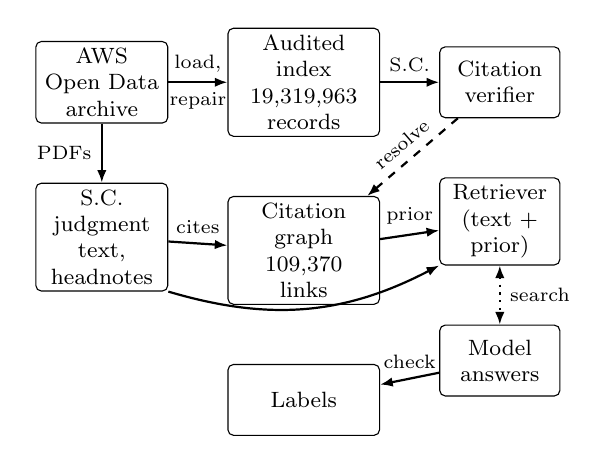
\begin{tikzpicture}[
  box/.style={draw, rounded corners=2pt, align=center, font=\footnotesize, minimum height=0.9cm, inner sep=2.5pt},
  arr/.style={-{Latex[length=1.6mm]}, thick},
  lbl/.style={font=\scriptsize, align=center}]
\node[box, text width=1.5cm] (aws) {AWS Open Data archive};
\node[box, text width=1.75cm, right=0.75cm of aws] (idx) {Audited index\\ \CorpusTotal{}\\ records};
\node[box, text width=1.35cm, right=0.75cm of idx] (ver) {Citation\\ verifier};
\node[box, text width=1.5cm, below=0.75cm of aws] (txt) {S.C. judgment text, headnotes};
\node[box, text width=1.75cm, below=0.75cm of idx] (graph) {Citation graph\\ \GraphEdges{}\\ links};
\node[box, text width=1.35cm, below=0.75cm of ver] (ret) {Retriever\\ (text + prior)};
\node[box, text width=1.35cm, below=0.75cm of ret] (llm) {Model\\ answers};
\node[box, text width=1.75cm, below=0.75cm of graph] (lab) {Labels};
\draw[arr] (aws) -- node[lbl, above] {load,} node[lbl, below] {repair} (idx);
\draw[arr] (idx) -- node[lbl, above] {S.C.} (ver);
\draw[arr] (aws) -- node[lbl, left] {PDFs} (txt);
\draw[arr] (txt) -- node[lbl, above] {cites} (graph);
\draw[arr, dashed] (ver) -- node[lbl, sloped, above] {resolve} (graph);
\draw[arr] (graph) -- node[lbl, above] {prior} (ret);
\draw[arr] (txt.south east) to[bend right=22] (ret.south west);
\draw[arr, {Latex[length=1.6mm]}-{Latex[length=1.6mm]}, dotted] (ret) -- node[lbl, right] {search} (llm);
\draw[arr] (llm) -- node[lbl, above] {check} (lab);
\end{tikzpicture}
\caption{Overview. The archive's metadata is loaded into an audited index; the verifier resolves citations and case names against its Supreme Court part. The text of every Supreme Court judgment yields headnotes and the citations each judgment makes, which the verifier resolves into a citation graph. The retriever searches headnotes by subject and ranks with the graph's citation counts. Model answers are checked by the verifier; in the search conditions the model queries the index or the retriever before answering.}
\label{fig:pipeline}
\end{figure}


\section{Related Work}
Dahl et al.\ found hallucination rates of 58\% (ChatGPT~4) to 88\% (Llama~2) on verifiable questions about United States federal cases \cite{dahl2024}, and commercial retrieval-augmented legal tools still hallucinate on 17--33\% of queries \cite{magesh2025}; detector benchmarks \cite{liu2026checks}, LegalCiteBench \cite{legalcitebench} and a study of substituted cases \cite{verma2026} also concern United States law. eyecite extracts United States citations \cite{eyecite} and CourtListener flags invalid ones \cite{courtlistenerapi}; our verifier plays that role for the Supreme Court of India, whose neutral and S.C.R. formats differ. Fowler et al.\ built the citation network of the United States Supreme Court \cite{fowler2007}; prior-case retrieval takes its labels from the citations in judgments \cite{joshi2023ucreat,farber2020}, and retrieval-augmented generation grounds a model in retrieved documents \cite{lewis2020rag}. Recent legal agents audit their citations \cite{lmars,parthenon,maat}. Indian resources include ILDC \cite{ildc}, IL-TUR \cite{iltur}, NyayaRAG \cite{nyayarag} and the Supreme Court's assistive tools SUVAS and SUPACE \cite{suvas,supace}; open-india-law releases text and embeddings for 12.8 million judgments and treats a citation graph as out of scope \cite{openindialaw}.

\section{An Open Index of Indian Judgments}
\label{sec:corpus}
The AWS Open Data registry hosts two CC-BY-4.0 datasets published by Dattam Labs: judgments of the Supreme Court from 1950 \cite{awssc} and of 25 High Courts \cite{awshc}, with structured metadata in Parquet and the judgments as PDFs. We load only the metadata into one PostgreSQL 17 table of \CorpusTotal{} records (\CorpusSC{} Supreme Court judgments and \CorpusHC{} High Court judgments and orders, \CorpusCourts{} courts, decided \CorpusYearMin{}--\CorpusYearMax), each with a link to its PDF in the archive, never the PDF.

\textbf{Audit and repair.} Records from the archive's ``mobile'' path store a bare file name where a bench-qualified path is needed, so their PDF link cannot be formed \cite{hcdatasetdoc}: \MobileTotal{} records in four High Courts (\MobilePct{} of the corpus), \MobileRecentPct{} decided in 2024--2026. The file name is no identity either: \CollideStems{} names occur in more than one bench, covering \CollideRows{} records, and in \CollideDiffBothPct{} of these the title and date both differ, so keying on the file name, as our first load did, silently overwrites at least \CollideLost{} records. We key on the case number (CNR), take the bench from the S3 key, and link a record only when its file exists in the archive's listing. This restores \MobileLinked{} links (\MobileLinkedPct); the other \MobileUnrecov{} records have no PDF in the archive. After repair \LinkedPct{} of all records carry a link. All \RecoveredChecked{} sampled restored links, all \NonmobileChecked{} sampled original High Court links (\NonmobileCourts{} courts) and all \SCLinksChecked{} sampled Supreme Court links resolve against the live archive, and for \UnresolvedChecked{} sampled unrecoverable records the expected file does not exist.

\begin{figure}[t]
\centering
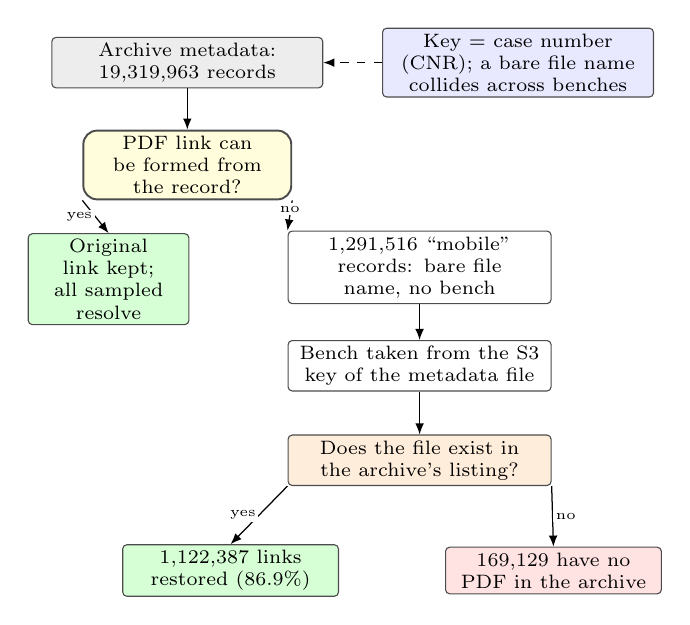
\begin{tikzpicture}[x=1cm,y=1cm]
\node[io, text width=3.3cm] (r1) at (1.95,5.5) {Archive metadata: \CorpusTotal{} records};
\node[db, text width=3.3cm] (r2) at (6.15,5.5) {Key = case number (CNR); a bare file name collides across benches};
\node[dec, text width=2.5cm] (r3) at (1.95,4.2) {PDF link can be formed from the record?};
\node[ok, text width=1.9cm] (r4) at (0.95,2.75) {Original link kept; all sampled resolve};
\node[st, text width=3.2cm] (r5) at (4.9,2.9) {\MobileTotal{} ``mobile'' records: bare file name, no bench};
\node[st, text width=3.2cm] (r6) at (4.9,1.65) {Bench taken from the S3 key of the metadata file};
\node[ch, text width=3.2cm] (r7) at (4.9,0.45) {Does the file exist in the archive's listing?};
\node[ok, text width=2.6cm] (r8) at (2.5,-0.95) {\MobileLinked{} links restored (\MobileLinkedPct)};
\node[wr, text width=2.6cm] (r9) at (6.6,-0.95) {\MobileUnrecov{} have no PDF in the archive};
\draw[ar] (r1)--(r3);
\draw[ar] (r3.south west)--node[lb,left]{yes}(r4.north);
\draw[ar] (r3.south east)--node[lb,above]{no}(r5.north west);
\draw[ar] (r5)--(r6); \draw[ar] (r6)--(r7);
\draw[ar] (r7.south west)--node[lb,left]{yes}(r8.north);
\draw[ar] (r7.south east)--node[lb,right]{no}(r9.north);
\draw[dar] (r2.west)--(r1.east);
\end{tikzpicture}
\caption{Auditing and repairing the archive's High Court links (\S\ref{sec:corpus}). Records are keyed on the case number, and a link is made only when its file exists in the archive's own listing.}
\label{fig:repair}
\end{figure}


\textbf{Supreme Court metadata.} Every one of the \CorpusSC{} judgments carries an S.C.R. citation and \SCwithNeutral{} a neutral citation \cite{scneutral}. Three properties matter for verification. The year field is the year of the S.C.R. volume, not of the decision, for \SCYearNe{} judgments (\SCYearNePct), so we use the decision date. \SCDupGroups{} neutral citations are attached to more than one record. And for each year from 1950 to 2013 except \INSCIncompleteList{} the index holds every neutral number from 1 to the year's maximum \cite{scneutral2}, so a missing number is unassigned for those \INSCCompleteCount{} years.

\section{Citation Verifier}
\label{sec:verifier}
The verifier takes a case name, a year and a citation string, as a model produced them, and decides whether they denote a real Supreme Court judgment in the index (Fig.~\ref{fig:verifier}). Neutral and S.C.R. citations are looked up exactly (a citation without a volume matches any volume of that series, year and page); SCC, AIR and other reports cannot be resolved against the index, so for them the name decides. Names are compared word by word: stop-words are dropped, abbreviations expanded, and each word is weighted by $\log(N/\mathrm{df})$ over the $N$ judgments \cite{sparckjones}. Two words match if they are equal or, for words of five or more letters, if their similarity ratio \cite{difflib} is at least 0.85, which accepts \emph{Keshavananda}/\emph{Kesavananda} but not \emph{Patil}/\emph{Patel}. The name score is the harmonic mean of the share of the cited name's weight that is matched ($p$) and of the judgment's ($r$), set to zero if $p<0.8$ so that an unmatched given name cannot be outweighed by words such as \emph{State}; a candidate must lie within a year of the stated year, and the threshold is $\tau=0.5$. VERIFIED establishes that the judgment exists near that year, not that it supports the proposition it is cited for. We developed the rules on the T4 answers of three models, reviewing a development sample of 56 decisions by hand, and then froze the verifier, recording hashes of its code, before the benchmark and the held-out audit of \S\ref{sec:audit}.

\begin{figure*}[t]
\centering
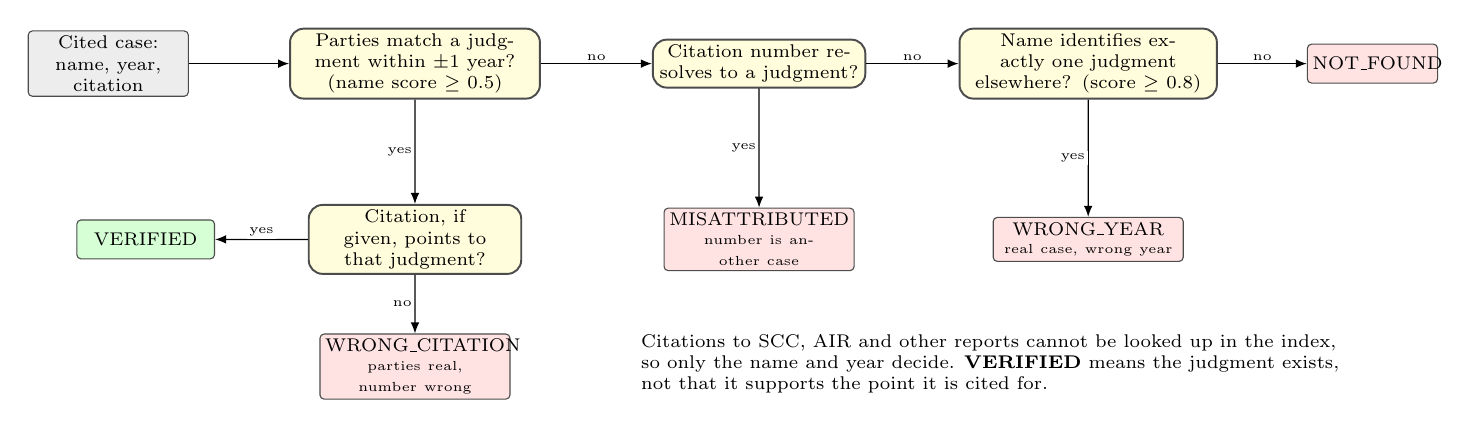
\begin{tikzpicture}[x=1cm,y=1cm,scale=0.95,transform shape]
\node[io, text width=2.0cm] (in) at (0,0) {Cited case: name, year, citation};
\node[dec, text width=3.2cm] (d1) at (4.1,0) {Parties match a judgment within $\pm$1 year? (name score $\ge$ 0.5)};
\node[dec, text width=2.7cm] (d3) at (8.7,0) {Citation number resolves to a judgment?};
\node[dec, text width=3.3cm] (d4) at (13.1,0) {Name identifies exactly one judgment elsewhere? (score $\ge$ 0.8)};
\node[wr, text width=1.6cm] (nf) at (16.9,0) {NOT\_FOUND};
\node[dec, text width=2.7cm] (d2) at (4.1,-2.35) {Citation, if given, points to that judgment?};
\node[ok, text width=1.7cm] (ve) at (0.5,-2.35) {VERIFIED};
\node[wr, text width=2.4cm] (wc) at (4.1,-4.05) {WRONG\_CITATION\\[-1pt]{\tiny parties real, number wrong}};
\node[wr, text width=2.4cm] (mi) at (8.7,-2.35) {MISATTRIBUTED\\[-1pt]{\tiny number is another case}};
\node[wr, text width=2.4cm] (wy) at (13.1,-2.35) {WRONG\_YEAR\\[-1pt]{\tiny real case, wrong year}};
\draw[ar] (in) -- (d1);
\draw[ar] (d1) -- node[lb,above]{no} (d3);
\draw[ar] (d3) -- node[lb,above]{no} (d4);
\draw[ar] (d4) -- node[lb,above]{no} (nf);
\draw[ar] (d1) -- node[lb,left]{yes} (d2);
\draw[ar] (d2) -- node[lb,above]{yes} (ve);
\draw[ar] (d2) -- node[lb,left]{no} (wc);
\draw[ar] (d3) -- node[lb,left]{yes} (mi);
\draw[ar] (d4) -- node[lb,left]{yes} (wy);
\node[font=\scriptsize, align=left, anchor=north west] at (7.0,-3.5) {Citations to SCC, AIR and other reports cannot be looked up in the index,\\so only the name and year decide. {\bfseries VERIFIED} means the judgment exists,\\not that it supports the point it is cited for.};
\end{tikzpicture}
\caption{How the verifier labels a citation (\S\ref{sec:verifier}). Each case a model cites ends in one of five labels; the audit of \S\ref{sec:audit} found \AuditPct{} of them correct.}
\label{fig:verifier}
\end{figure*}


\section{Citation Graph}
\label{sec:graph}
We downloaded the PDF of every Supreme Court judgment and extracted its text layer with PyMuPDF (the reports carry an embedded OCR layer): \GraphTextOK{} of \CorpusSC{} were extracted. Each judgment opens with the reporter's headnote, which we cut at the jurisdiction line and keep to 3{,}000 characters. We find every reporter citation (S.C.R., neutral, SCC, Supreme Court AIR) and resolve each distinct pair of citing judgment and citation in three tiers (Fig.~\ref{fig:graphretr}A): the number, a parallel number written beside an SCC or AIR citation, and the name and year through the frozen verifier, accepted only if exactly one judgment matches. A pair whose number and name disagree is dropped. We developed the extractor on a pilot of \PilotN{} judgments and ran it once over the corpus.

It found \GraphUnits{} distinct pairs, of which \GraphResolved{} (\GraphResolvedPct) were resolved, giving \GraphEdges{} distinct links between \GraphCiting{} citing and \GraphCited{} cited judgments: \GraphCitedPct{} of reported judgments are cited by a later one. Where a citation carries a number and a name that can both be resolved, the name and year alone reach the number's record in \GraphNameSamePct{} of \GraphNamePrecN{} cases, a label-free estimate of the precision of name-only links; another \GraphNameLoosePct{} reach a different record with matching parties, such as another order in the same case. Only \GraphLater{} links (\GraphLaterPct) point to a later judgment, which is impossible, and all \GraphCheckN{} name-only links we drew for a hand check were correct. The most cited judgments are \emph{Maneka Gandhi v.\ Union of India} (\GraphTopOneN{} citing judgments), \emph{Kesavananda Bharati} (\GraphTopTwoN) and \emph{Sharad Birdhi Chand Sarda} (\GraphTopThreeN), and \GraphLandmarkCited{} of the \GraphLandmarkN{} landmark judgments we chose before the graph existed are cited at least once.

\section{Retrieval}
\label{sec:retrieval}
We index the title and headnote of every judgment two ways: BM25 \cite{robertson2009} over unigrams and bigrams, and dense retrieval with the open multilingual model bge-m3 \cite{chen2024m3}. The hybrid retriever takes the union of the top 300 of each and adds their scores after normalising each; a citation prior adds the normalised $\log(1+c)$, where $c$ is the number of judgments in the graph that cite the candidate (Fig.~\ref{fig:graphretr}B). Weights are chosen on a development split. The graph also supplies relevance labels without annotation \cite{farber2020,joshi2023ucreat}: for each of \RecNTest{} held-out judgments that cite at least \RecMinTargets{} earlier ones, the query is its headnote with every citation and case name removed, the targets are the judgments it cites, and only earlier judgments and citations made before its date are used.

The hybrid retriever with the prior places \RecHybridPriorRTenPct{} of the cited judgments in its top ten (hybrid alone \RecHybridRTen, BM25 \RecBmRTen, dense \RecDenseRTen, popularity alone \RecPopRTen), a relative gain of \RecPriorRelGain{} (paired bootstrap 95\% CI of the difference \RecDiffPriorCI). Searched with the question text, it returns a judgment that decided the question among its top three for \QHybridPriorHitThree{} of the \NumTopics{} legal questions (\QHybridHitThree{} without the prior), while no model named such a judgment from memory for more than \RefClosedLlama. The questions were written around landmark judgments, which favours the prior; the recommendation experiment has no such bias.

\begin{figure*}[t]
\centering
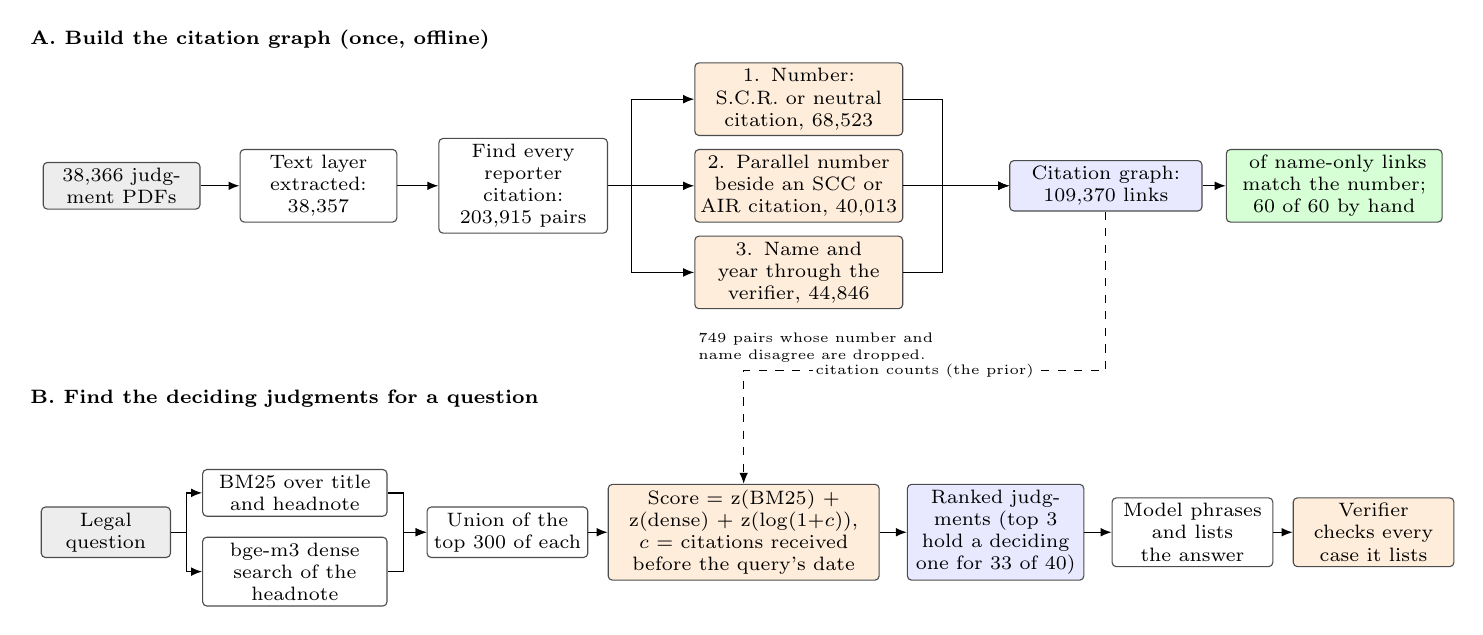
\begin{tikzpicture}[x=1cm,y=1cm]
% lane 1: build the graph
\node[ttl, anchor=west] at (-0.2,4.15) {A. Build the citation graph (once, offline)};
\node[io, text width=1.85cm] (a1) at (1.0,2.3) {\CorpusSC{} judgment PDFs};
\node[st, text width=1.85cm] (a2) at (3.5,2.3) {Text layer extracted: \GraphTextOK{}};
\node[st, text width=2.0cm] (a3) at (6.1,2.3) {Find every reporter citation: \GraphUnits{} pairs};
\node[ch, text width=2.5cm] (t1) at (9.6,3.4) {1. Number: S.C.R. or neutral citation, \GraphExact{}};
\node[ch, text width=2.5cm] (t2) at (9.6,2.3) {2. Parallel number beside an SCC or AIR citation, \GraphParallel{}};
\node[ch, text width=2.5cm] (t3) at (9.6,1.2) {3. Name and year through the verifier, \GraphName{}};
\node[db, text width=2.3cm] (a5) at (13.5,2.3) {Citation graph: \GraphEdges{} links};
\node[ok, text width=2.6cm] (a6) at (16.4,2.3) {\GraphNameSamePct{} of name-only links match the number; 60 of 60 by hand};
\node[font=\tiny, text width=3.4cm, align=left, anchor=north west] at (8.2,0.55) {\GraphConflict{} pairs whose number and name disagree are dropped.};
\draw[ar] (a1)--(a2); \draw[ar] (a2)--(a3);
\draw[ar] (a3.east)--++(0.3,0)|-(t1.west); \draw[ar] (a3.east)--(t2.west); \draw[ar] (a3.east)--++(0.3,0)|-(t3.west);
\draw[ar] (t1.east)--++(0.5,0)|-(a5.west); \draw[ar] (t2.east)--(a5.west); \draw[ar] (t3.east)--++(0.5,0)|-(a5.west);
\draw[ar] (a5)--(a6);
% lane 2: answer a question
\node[ttl, anchor=west] at (-0.2,-0.4) {B. Find the deciding judgments for a question};
\node[io, text width=1.5cm] (b1) at (0.8,-2.1) {Legal question};
\node[st, text width=2.2cm] (b2) at (3.2,-1.6) {BM25 over title and headnote};
\node[st, text width=2.2cm] (b3) at (3.2,-2.6) {bge-m3 dense search of the headnote};
\node[st, text width=1.9cm] (b4) at (5.9,-2.1) {Union of the top 300 of each};
\node[ch, text width=3.3cm] (b5) at (8.9,-2.1) {Score = z(BM25) + z(dense) + z($\log(1{+}c)$), $c$ = citations received before the query's date};
\node[db, text width=2.1cm] (b6) at (12.1,-2.1) {Ranked judgments (top 3 hold a deciding one for \QHybridPriorHitThree{} of \NumTopics{})};
\node[st, text width=1.9cm] (b7) at (14.6,-2.1) {Model phrases and lists the answer};
\node[ch, text width=1.9cm] (b8) at (16.9,-2.1) {Verifier checks every case it lists};
\draw[ar] (b1.east)--++(0.2,0)|-(b2.west); \draw[ar] (b1.east)--++(0.2,0)|-(b3.west);
\draw[ar] (b2.east)--++(0.2,0)|-(b4.west); \draw[ar] (b3.east)--++(0.2,0)|-(b4.west);
\draw[ar] (b4)--(b5); \draw[ar] (b5)--(b6); \draw[ar] (b6)--(b7); \draw[ar] (b7)--(b8);
\draw[dar] (a5.south)--(13.5,-0.05)--(8.9,-0.05)--(b5.north);
\node[lb] at (11.2,-0.05) {citation counts (the prior)};
\end{tikzpicture}
\caption{From judgment text to checked authorities. (A) Every Supreme Court judgment is read for the citations it makes, and each is resolved in three tiers (\S\ref{sec:graph}). (B) A question is searched by subject, re-ranked with the graph's citation counts, and the model's answer is checked (\S\ref{sec:retrieval}).}
\label{fig:graphretr}
\end{figure*}


\section{How Small Models Cite}
\label{sec:setup}
The benchmark uses \NumJudgments{} Supreme Court judgments (\NumLandmark{} landmarks identified by name and \NumRandom{} sampled at random, 1950--2023) and five tasks. T1 asks for the judgment reported at a citation (\NumTOne{} items); T2 asks the same for citations that cannot exist (\NumTTwo{} items; declining is correct); T3 asks for the citations of a judgment given its parties and date (\NumTThree{} items); T4 asks for up to three leading authorities on each of \NumTopics{} legal questions, each case labelled by the verifier; T5 gives the model the verifier's findings on its T4 answer and asks it to revise. For T4 we record reference answers, the judgments that decided each question (\NumRefJudgments{} index records, including earlier decisions later overruled), compiled after the closed-book runs and before the search runs and hashed; a question counts as answered if a listed case matches one. We evaluate four open-weight models that fit an 8\,GB laptop GPU, in 4-bit quantisation through Ollama \cite{ollama}: Llama~3.1 8B \cite{llama3}, Qwen3 8B \cite{qwen3}, Gemma~3 4B \cite{gemma3} and Qwen2.5-VL 7B \cite{qwen25vl}, with one system prompt, temperature~0, a fixed seed and a JSON schema. In the name-search condition a model has two tools over the index metadata (search by party names, lookup by citation); in the two topic-search conditions its tool is the retriever, without and with the citation prior. Each condition was run once, after the code and the reference answers were frozen by hash.

\begin{figure}[t]
\centering
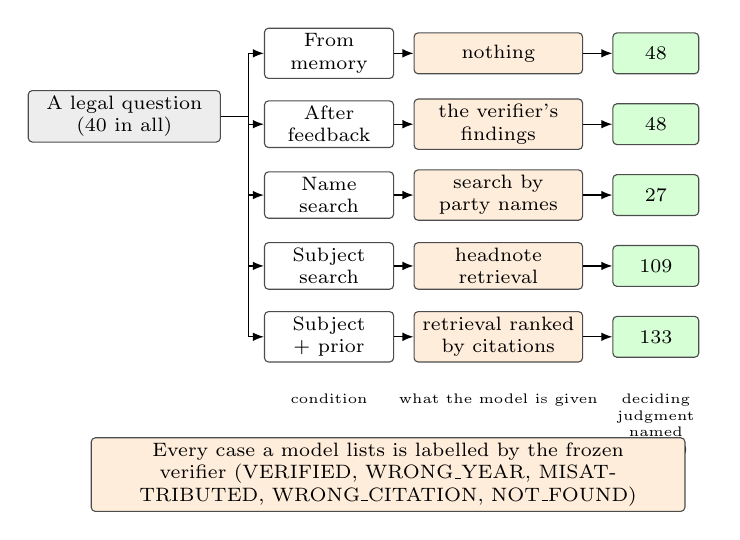
\begin{tikzpicture}[x=1cm,y=1cm]
\node[io, text width=2.3cm] (q) at (0.85,4.55) {A legal question (\NumTopics{} in all)};
\foreach \i/\y/\n/\u/\c in {1/5.35/{From memory}/{nothing}/{\FigNamedA},
                            2/4.45/{After feedback}/{the verifier's findings}/{\FigNamedB},
                            3/3.55/{Name search}/{search by party names}/{\FigNamedC},
                            4/2.65/{Subject search}/{headnote retrieval}/{\FigNamedD},
                            5/1.75/{Subject + prior}/{retrieval ranked by citations}/{\FigNamedE}} {
  \node[st, text width=1.5cm] (c\i) at (3.45,\y) {\n};
  \node[ch, text width=2.0cm] (u\i) at (5.6,\y) {\u};
  \node[ok, text width=0.95cm] (o\i) at (7.6,\y) {\c};
  \draw[ar] (c\i)--(u\i); \draw[ar] (u\i)--(o\i);
}
\draw[ar] (q.east) -- ++(0.35,0) |- (c1.west);
\draw[ar] (q.east) -- ++(0.35,0) |- (c2.west);
\draw[ar] (q.east) -- ++(0.35,0) |- (c3.west);
\draw[ar] (q.east) -- ++(0.35,0) |- (c4.west);
\draw[ar] (q.east) -- ++(0.35,0) |- (c5.west);
\node[font=\tiny, anchor=north] at (3.45,1.15) {condition};
\node[font=\tiny, anchor=north] at (5.6,1.15) {what the model is given};
\node[font=\tiny, anchor=north, text width=1.2cm, align=center] at (7.6,1.15) {deciding judgment named (of \FigAll{})};
\node[ch, text width=7.4cm] (v) at (4.2,0.0) {Every case a model lists is labelled by the frozen verifier (VERIFIED, WRONG\_YEAR, MISATTRIBUTED, WRONG\_CITATION, NOT\_FOUND)};
\end{tikzpicture}
\caption{The five conditions of the benchmark (\S\ref{sec:setup}). Each of four models answered the same questions under each; the right-hand figure is the number of model--question pairs in which a case that decided the question was named.}
\label{fig:conditions}
\end{figure}


\section{Results: What Retrieval Changes}
\label{sec:results}
\textbf{From memory.} Llama and Gemma answered almost everything and were almost always wrong: Llama identified \TOneCorrectLlama{} of the \TOneN{} real citations, Gemma none, and both named a judgment for nearly every fabricated citation (\TTwoNamedLlama{} and \TTwoNamedGemma{} of 60; Table~\ref{tab:t1t2}). The two Qwen models declined all 262 questions. No model identified more than \BestTOneCorrect{} of \TOneN{} real citations, and given the parties and date they supplied \TThreeCorrectAll{} correct citations of \TThreeAskedAll{} requested. Asked for authorities, the models cited between \TFourCasesMin{} and \TFourCasesMax{} cases each, of which only \TFourVerifiedRange{} could be verified (Table~\ref{tab:t4}); they cited almost only the SCC and AIR reports, which the index cannot resolve, so those labels rest on party names and year. On a fresh stratified sample of \AuditN{} T4 decisions judged by hand the verifier was right in \AuditCorrect{} (\AuditPct) \label{sec:audit}, and of the \AuditNFN{} audited NOT\_FOUND cases \AuditNFFab{} named parties that match no Supreme Court judgment in any year.

\textbf{Feedback and search by name.} Telling a model what the verifier found removed the flagged cases (NOT\_FOUND fell from \TFiveNFBeforeAll{} to \TFiveNFAfterAll; Table~\ref{tab:t5}) but added none: \TFiveRepeatedAll{} of the \TFiveCasesAfterAll{} cases in the revised lists were repeated from the first answers. Name search almost eliminated cases the index cannot find (\NFClosedAll{} to \NFSearchAll), but fewer answers contained a deciding judgment (\RefSearchAll{} of \RefQuestionsAll{} against \RefClosedAll): the models searched with the question's words, the tool matched party names, and the judgments it returned exist but decide nothing, such as \emph{Fair Air Engineers v.\ N.K.\ Modi} for a question \emph{Maneka Gandhi} answers.

\textbf{Search by subject.} With the retriever the models named a deciding judgment in \RefAllTopic{} of \RefQuestionsAll{} pairs, and in \RefAllTopicPrior{} with the citation prior (Fig.~\ref{fig:results}, Table~\ref{tab:conds}); counting each question once, \SignClosedTopicPriorBetter{} questions were answered by more models than from memory and \SignClosedTopicPriorWorse{} by fewer (exact sign test, $p$~\SignClosedTopicPriorP). \VerPctAllTopicPrior{} of the \CasesAllTopicPrior{} cases they listed were verified, against \VerPctAllClosed{} from memory. The gain was largest for the model that knew least: Qwen2.5-VL named a deciding judgment for \RefClosedQwenVL{} questions from memory and \RefTopicPriorQwenVL{} with the retriever. The models listed mostly what the search had shown them, and the retriever's top three alone answer \QHybridPriorHitThree{} questions, about as many as the models do (\RefTopicPriorGemma--\RefTopicPriorLlama): the index guarantees existence, the retriever and the graph supply relevance, and the model at most phrases and orders the result.

\begin{table}[t]
\caption{Deciding judgments named and cases not found, by model and condition (\S\ref{sec:setup}). Ref.\ is the number of the \NumTopics{} questions for which a case that decided the question was named; N.F.\ is the number of listed cases the verifier could not find.}
\label{tab:conds}
\centering
\scriptsize
\setlength{\tabcolsep}{2pt}
\resizebox{\columnwidth}{!}{\begin{tabular}{lrrrrrrrrrr}
\toprule
 & \multicolumn{2}{c}{From memory} & \multicolumn{2}{c}{After feedback} & \multicolumn{2}{c}{Name search} & \multicolumn{2}{c}{Topic search} & \multicolumn{2}{c}{Topic + prior} \\
\cmidrule(lr){2-3}\cmidrule(lr){4-5}\cmidrule(lr){6-7}\cmidrule(lr){8-9}\cmidrule(lr){10-11}
Model & Ref. & N.F. & Ref. & N.F. & Ref. & N.F. & Ref. & N.F. & Ref. & N.F. \\
\midrule
Llama 3.1 8B & 24 & 42 & 24 & 4 & 10 & 4 & 29 & 2 & 35 & 1 \\
Qwen3 8B & 13 & 49 & 13 & 1 & 12 & 1 & 24 & 0 & 33 & 0 \\
Gemma 3 4B & 8 & 81 & 8 & 16 & 5 & 1 & 27 & 0 & 32 & 0 \\
Qwen2.5-VL 7B & 3 & 67 & 3 & 31 & 0 & 2 & 29 & 0 & 33 & 0 \\
\midrule
All four & 48 & 239 & 48 & 52 & 27 & 8 & 109 & 2 & 133 & 1 \\
\bottomrule
\end{tabular}
}
\end{table}

\textbf{Existence and authority are different checks.} A verifier over names and citations catches fabricated cases, and feedback from it or search over it removed almost all of them, but it did not help the models find the judgment that decides a question, and name search made that rarer. A real but irrelevant judgment passes an existence check, so a system that shows only ``verified'' citations can look more reliable while citing worse authorities. Finding authority needs what the metadata lacks: what each judgment decided, which the headnote supplies, and which judgments the Court itself relies on, which the graph supplies. The prior favours old and frequently cited judgments, including ones later overruled such as \emph{A.D.M.\ Jabalpur}, which a lawyer must cite as overruled.

\textbf{What remains unchecked.} Neither the verifier nor the retriever checks that a judgment supports the proposition it is cited for, which needs its reasoning and is hard even for strong models \cite{verma2026}, and the graph records that one judgment cites another, not whether it follows or overrules it. The graph and verifier cover the Supreme Court only: the High Court records have no citation fields (none of \HCMetaN{} sampled records had one), so extracting their citations needs the judgments themselves, about \HCTotalTB\,TB of PDFs by our sample, which we did not download.

\textbf{Limits of the benchmark.} We evaluated four open-weight models of 4 to 8 billion parameters in 4-bit quantisation with one prompt and greedy decoding; larger and hosted models, including those VakilBuddy calls through OpenRouter, may behave differently and are untested. The benchmark is small (\NumJudgments{} judgments, \NumTopics{} questions), and the audit labels, reference answers and hand checks come from a single annotator, so we cannot report inter-annotator agreement; the reference answers were compiled after the closed-book runs and, being landmarks, favour the citation prior.

\begin{figure}[t]
\centering
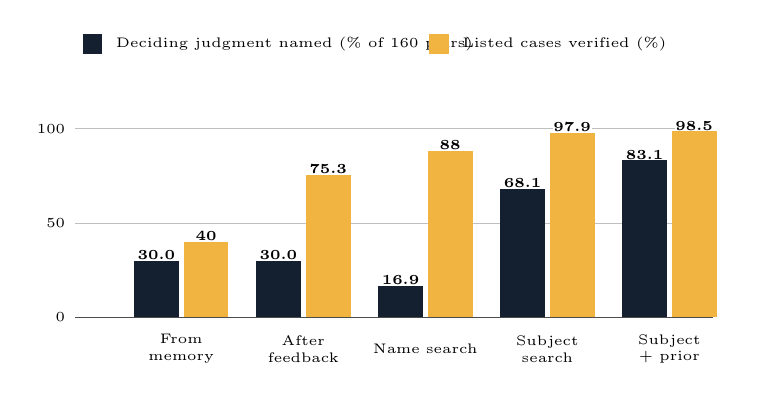
\begin{tikzpicture}[x=1cm,y=1cm]
% bars: heights come from the generated numbers (percent of 160 model--question pairs; percent of listed cases verified)
\def\H{2.4}            % height of 100 percent, in cm
\pgfmathsetmacro{\k}{\H/100}
\foreach \p in {0,50,100} {
  \pgfmathsetmacro{\yy}{\p*\k}
  \draw[black!25, line width=0.3pt] (0.2,\yy)--(8.3,\yy); \node[font=\tiny, left] at (0.2,\yy) {\p};
}
\foreach \i/\lab/\a/\b in {1/{From memory}/\FigPctA/\FigVerA, 2/{After feedback}/\FigPctB/\FigVerB, 3/{Name search}/\FigPctC/\FigVerC, 4/{Subject search}/\FigPctD/\FigVerD, 5/{Subject + prior}/\FigPctE/\FigVerE} {
  \pgfmathsetmacro{\ha}{\a*\k}
  \pgfmathsetmacro{\hb}{\b*\k}
  \pgfmathsetmacro{\cx}{1.55*\i}
  \node[font=\tiny, align=center, text width=1.4cm] at (\cx, -0.4) {\lab};
  \fill[navy] (\cx-0.6,0) rectangle (\cx-0.03,\ha);
  \fill[gold] (\cx+0.03,0) rectangle (\cx+0.6,\hb);
  \node[font=\tiny\bfseries, above, fill=white, inner sep=0.3pt] at (\cx-0.315,\ha) {\a};
  \node[font=\tiny\bfseries, above, fill=white, inner sep=0.3pt] at (\cx+0.315,\hb) {\b};
}
\draw[black!70] (0.2,0)--(8.3,0);
\fill[navy] (0.3,3.35) rectangle (0.55,3.6); \node[font=\tiny, anchor=west] at (0.6,3.475) {Deciding judgment named (\% of \FigAll{} pairs)};
\fill[gold] (4.7,3.35) rectangle (4.95,3.6); \node[font=\tiny, anchor=west] at (5.0,3.475) {Listed cases verified (\%)};
\end{tikzpicture}
\caption{What search and the citation graph change for four small open-weight models (\S\ref{sec:results}). Existence checks (feedback, name search) raise the share of verified cases, but only search by subject, ranked with the citation prior, raises the share of questions answered with a deciding judgment.}
\label{fig:results}
\end{figure}


\begin{table}[t]
\caption{Identifying a judgment from its citation. T1: \NumTOne{} real citations. T2: \NumTTwo{} citations that cannot exist. Corr.\ = named the right judgment; Named = named any judgment for a fabricated citation; Decl.\ = declined; Inv.\ = invalid output. ``Qwen3 8B think'' is the same model with reasoning enabled.}
\label{tab:t1t2}
\centering
\scriptsize
\setlength{\tabcolsep}{2.5pt}
\begin{tabular}{lrrrrrrr}
\toprule
& \multicolumn{4}{c}{T1: real citation (\%)} & \multicolumn{3}{c}{T2: fabricated (\%)} \\
\cmidrule(lr){2-5}\cmidrule(lr){6-8}
Model & Corr. & Wrong & Decl. & Inv. & Named & Decl. & Inv. \\
\midrule
Llama 3.1 8B & 0.5 & 99.0 & 0.0 & 0.5 & 98.3 & 0.0 & 1.7 \\
Qwen3 8B & 0.0 & 0.0 & 100.0 & 0.0 & 0.0 & 100.0 & 0.0 \\
Qwen3 8B think & 1.0 & 14.4 & 83.2 & 1.5 & 10.0 & 88.3 & 1.7 \\
Gemma 3 4B & 0.0 & 100.0 & 0.0 & 0.0 & 100.0 & 0.0 & 0.0 \\
Qwen2.5-VL 7B & 0.0 & 0.0 & 100.0 & 0.0 & 0.0 & 100.0 & 0.0 \\
\bottomrule
\end{tabular}

\end{table}

\begin{table}[t]
\caption{T5: the T4 answers that contained an unverified case (Q), before and after the model revised them with the verifier's feedback.}
\label{tab:t5}
\centering
\scriptsize
\setlength{\tabcolsep}{2.5pt}
\begin{tabular}{lrrrrrrr}
\toprule
& & \multicolumn{2}{c}{Cases} & \multicolumn{2}{c}{Verified (\%)} & \multicolumn{2}{c}{Not found} \\
\cmidrule(lr){3-4}\cmidrule(lr){5-6}\cmidrule(lr){7-8}
Model & Q & Before & After & Before & After & Before & After \\
\midrule
Llama 3.1 8B & 30 & 87 & 48 & 49.4 & 87.5 & 42 & 4 \\
Qwen3 8B & 29 & 84 & 27 & 30.9 & 92.6 & 49 & 1 \\
Gemma 3 4B & 37 & 111 & 40 & 19.8 & 52.5 & 81 & 16 \\
Qwen2.5-VL 7B & 35 & 87 & 39 & 9.2 & 20.5 & 67 & 31 \\
\bottomrule
\end{tabular}

\end{table}

\begin{table}[t]
\caption{T4: every case cited for \NumTopics{} legal questions, by verifier label. Ver.\ = VERIFIED (with Wilson 95\% interval), W.Yr.\ = WRONG\_YEAR, W.Cit.\ = WRONG\_CITATION, Misatt.\ = MISATTRIBUTED, N.F.\ = NOT\_FOUND.}
\label{tab:t4}
\centering
\scriptsize
\setlength{\tabcolsep}{2.5pt}
\begin{tabular}{lrrrrrrr}
\toprule
& & \multicolumn{6}{c}{Share of cited cases (\%)} \\
\cmidrule(lr){3-8}
Model & Cases & Ver. & 95\% CI & W.Yr. & W.Cit. & Misatt. & N.F. \\
\midrule
Llama 3.1 8B & 114 & 61.4 & 52--70 & 1.8 & 0.0 & 0.0 & 36.8 \\
Qwen3 8B & 117 & 50.4 & 42--59 & 7.7 & 0.0 & 0.0 & 41.9 \\
Qwen3 8B think & 94 & 35.1 & 26--45 & 4.3 & 0.0 & 0.0 & 60.6 \\
Gemma 3 4B & 117 & 23.9 & 17--32 & 6.8 & 0.0 & 0.0 & 69.2 \\
Qwen2.5-VL 7B & 102 & 22.5 & 16--32 & 0.0 & 0.0 & 11.8 & 65.7 \\
\bottomrule
\end{tabular}

\end{table}



\clearpage
\section{VakilBuddy: Architecture}
\label{sec:system}
The findings above answer three weaknesses of ordinary legal assistants: single-turn answers, similarity without authority, and no independent check. They give three design principles. \emph{The index, not the model, decides what exists}: every citation is looked up and model text is checked against sources before it is shown. \emph{Authority comes from the record}: a draft may cite only the judgments the advocate pinned, and the citation graph, not text similarity alone, ranks what to pin. \emph{The advocate decides}: work moves through stages with an approval gate, and the workspace files and sends nothing.

VakilBuddy is a prototype litigation workspace organised around a \emph{matter} (a case file); Fig.~\ref{fig:arch} shows its parts. The workspace runs in the advocate's browser and keeps a matter's data in browser storage. A small server serves the page, builds model prompts, applies the source checks and holds the model key, which is never returned to the browser. Model requests go to OpenRouter \cite{openrouter} or any OpenAI-compatible endpoint. A separate case-law API answers searches and exact lookups over the index of \S\ref{sec:corpus}. A court-status service, with a cache, per-customer keys, rate limits and a markup-drift check, answers from saved sample pages in this prototype. The verifier, graph and retriever of \S\ref{sec:verifier}--\S\ref{sec:retrieval} are research code on the same database; the workspace does not call them yet and uses a simpler lookup (\S\ref{sec:checks}). Table~\ref{tab:features} lists what the workspace does today. Features marked ``model'' call a language model and pass its output through the checks of \S\ref{sec:checks}; the others are deterministic.

\begin{figure*}[t]
\centering
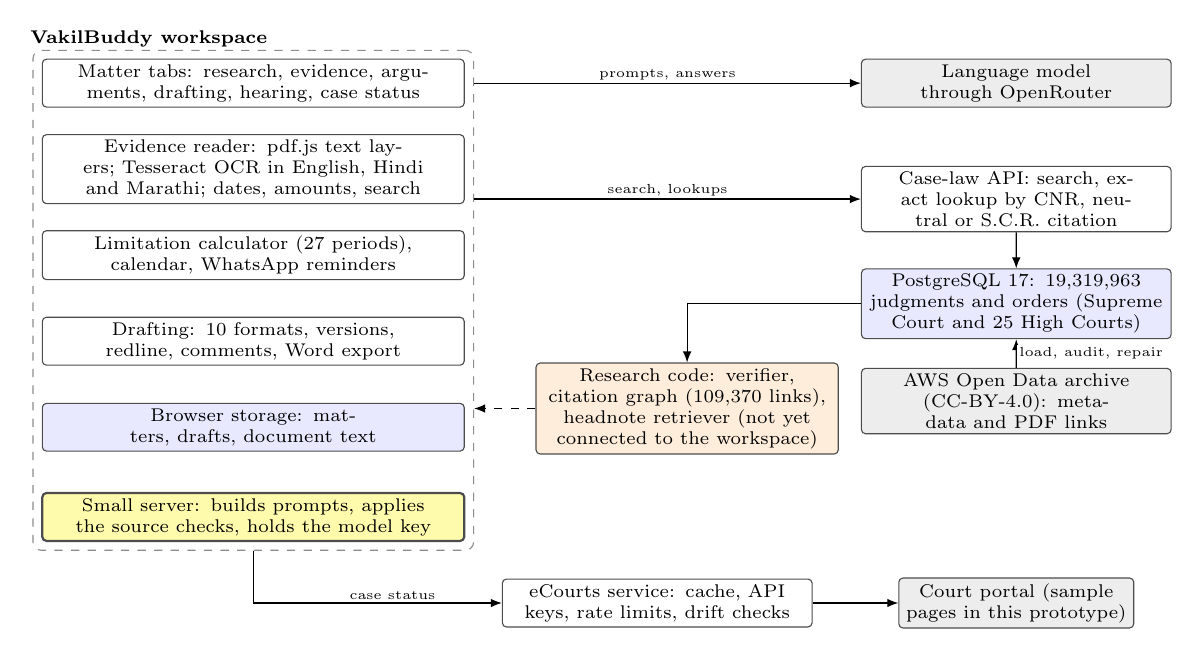
\begin{tikzpicture}[x=1cm,y=1cm,scale=0.95,transform shape]
% the workspace: browser modules and the small server
\node[st, text width=5.5cm] (m1) at (3.2,5.4) {Matter tabs: research, evidence, arguments, drafting, hearing, case status};
\node[st, text width=5.5cm] (m2) at (3.2,4.25) {Evidence reader: pdf.js text layers; Tesseract OCR in English, Hindi and Marathi; dates, amounts, search};
\node[st, text width=5.5cm] (m3) at (3.2,3.1) {Limitation calculator (\CasePeriods{} periods), calendar, WhatsApp reminders};
\node[st, text width=5.5cm] (m4) at (3.2,1.95) {Drafting: \CaseFormats{} formats, versions, redline, comments, Word export};
\node[db, text width=5.5cm] (m5) at (3.2,0.8) {Browser storage: matters, drafts, document text};
\node[hu, text width=5.5cm] (m6) at (3.2,-0.4) {Small server: builds prompts, applies the source checks, holds the model key};
\node[grp, fit=(m1)(m2)(m3)(m4)(m5)(m6), label={[ttl, anchor=south west, xshift=-2pt]north west:VakilBuddy workspace}] (ws) {};
% services
\node[io, text width=4.0cm] (llm) at (13.4,5.4) {Language model through OpenRouter};
\node[st, text width=4.0cm] (api) at (13.4,3.85) {Case-law API: search, exact lookup by CNR, neutral or S.C.R. citation};
\node[db, text width=4.0cm] (pg) at (13.4,2.45) {PostgreSQL 17: \CorpusTotal{} judgments and orders (Supreme Court and 25 High Courts)};
\node[io, text width=4.0cm] (aws) at (13.4,1.15) {AWS Open Data archive (CC-BY-4.0): metadata and PDF links};
\node[st, text width=4.0cm] (ec) at (8.6,-1.55) {eCourts service: cache, API keys, rate limits, drift checks};
\node[io, text width=3.0cm] (portal) at (13.4,-1.55) {Court portal (sample pages in this prototype)};
\node[ch, text width=3.9cm] (rs) at (9.0,1.05) {Research code: verifier, citation graph (\GraphEdges{} links), headnote retriever (not yet connected to the workspace)};
\draw[ar] (ws.east |- m1) -- node[lb, above]{prompts, answers} (llm.west |- m1);
\draw[ar] (ws.east |- api) -- node[lb, above, pos=0.5]{search, lookups} (api.west);
\draw[ar] (api) -- (pg);
\draw[ar] (aws) -- node[lb, right]{load, audit, repair} (pg);
\draw[ar] (ws.south) |- node[lb, above, pos=0.78]{case status} (ec.west);
\draw[ar] (ec) -- (portal);
\draw[ar] (pg.west) -| (rs.north);
\draw[dar] (rs.west) -- (ws.east |- rs.west);
\end{tikzpicture}
\caption{Architecture of VakilBuddy as built. The workspace runs in the advocate's browser with a small server; the case-law API serves the index of \S\ref{sec:corpus}; model requests go to OpenRouter; the court-status service answers from sample pages. The verifier, graph and retriever of \S\ref{sec:verifier}--\S\ref{sec:retrieval} are research code that the workspace does not yet call.}
\label{fig:arch}
\end{figure*}


\begin{table*}[t]
\caption{What the workspace does today, and where a language model is involved.}
\label{tab:features}
\centering
\footnotesize
\setlength{\tabcolsep}{4pt}
\renewcommand{\arraystretch}{1.08}
\begin{tabular}{@{}>{\raggedright\arraybackslash}p{1.35in}>{\raggedright\arraybackslash}p{3.9in}>{\raggedright\arraybackslash}p{1.35in}>{\raggedright\arraybackslash}p{0.45in}@{}}
\toprule
Feature & What it does & Built from & Model \\
\midrule
Case-law search & Exact lookup by CNR, neutral or S.C.R. citation; full-text and typo-tolerant search; filters by court, year and outcome & the index (\S\ref{sec:corpus}) & no \\
Citation check and pinned authorities & Finds the citations and case names in a text and looks each up; pins the judgments a matter relies on, each with a note of what for & the index & no \\
Evidence reading & Text, Word and PDF text layers; OCR in English, Hindi and Marathi; dates, amounts, search, possible inconsistencies & pdf.js, Tesseract & no \\
Chronology, cross-examination questions, witness comparison & Dated events and questions from the documents; positions that differ between witnesses & the matter's documents & model \\
Arguments & Points linked to pinned authorities; the other side's best answer to each & pinned authorities & model \\
Drafting & \CaseFormats{} formats filled from the record (Manual); sections written by a model that may cite only pinned authorities (Auto) & the record, pinned authorities & Auto \\
Para-wise reply & Numbers the other side's paragraphs; builds the reply from a stance for each, leaving the substance blank & the plaint or notice & no \\
Review and export & Versions, word-level redline, comments, approval, Word export with court-rule profiles & drafts & no \\
Limitation and reminders & \CasePeriods{} periods with their sources; counting by s.\,12 and s.\,4; saved dates; WhatsApp text the advocate sends & the statutes & no \\
Court status & Case record by CNR; an order digest; preparation for the next listing & the court-status service (sample data) & digest \\
\bottomrule
\end{tabular}
\end{table*}

\section{Workflow and the Approval Gate}
\label{sec:workflow}
A matter moves through the stages of Fig.~\ref{fig:flow}. Intake turns the advocate's account into a matter, research pins authorities, evidence is read and a chronology built, and arguments link points to authorities. Drafting starts from the matter's own record: pinned authorities, chronology and documents flow into drafts (Fig.~\ref{fig:pair1}a), so a fact or an authority is entered once. A draft is either \emph{Draft} or \emph{Approved} (Fig.~\ref{fig:pair1}b). Approval warns if review comments are open, saves a version and writes an audit-trail entry; an approved draft is locked, and a Word file or a print can be made only from an approved draft. Versions (the latest twelve) are saved when a draft is made, before an AI draft replaces text, when the advocate saves and on approval, and a word-level redline compares any two. This is the duty of care an advocate already owes the court \cite{gummadi}: a flagged citation is corrected by the advocate and never rewritten automatically.

\begin{figure*}[t]
\centering
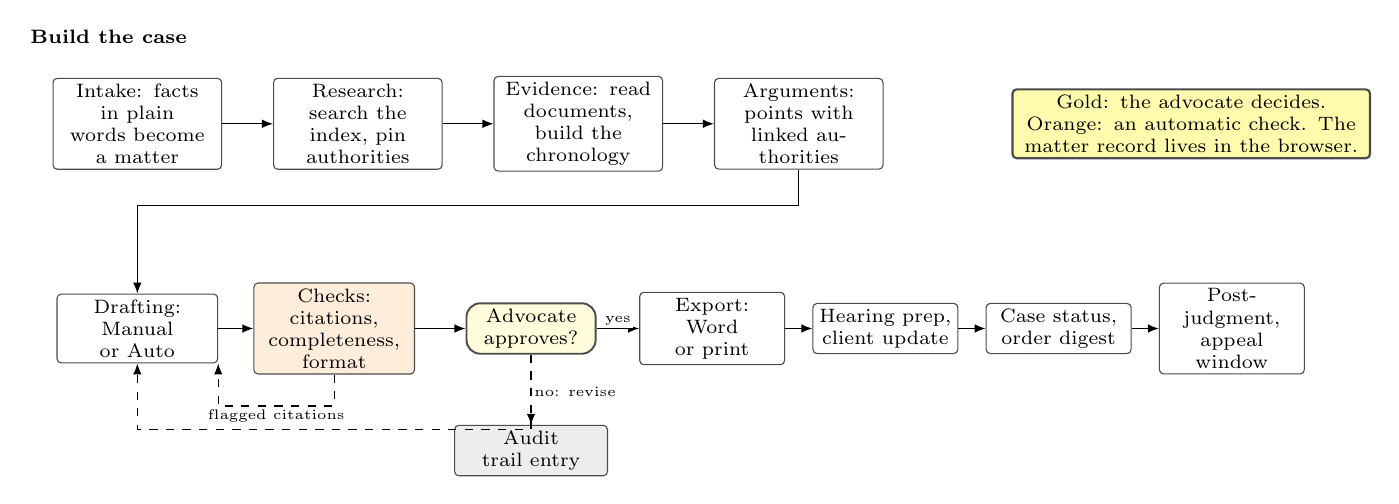
\begin{tikzpicture}[x=1cm,y=1cm]
% row 1: build the case
\node[ttl, anchor=west] at (-0.3,3.6) {Build the case};
\node[st, text width=2.0cm] (a1) at (1.1,2.5) {Intake: facts in plain words become a matter};
\node[st, text width=2.0cm] (a2) at (3.9,2.5) {Research: search the index, pin authorities};
\node[st, text width=2.0cm] (a3) at (6.7,2.5) {Evidence: read documents, build the chronology};
\node[st, text width=2.0cm] (a4) at (9.5,2.5) {Arguments: points with linked authorities};
\node[hu, text width=4.4cm, anchor=west] (lg) at (12.2,2.5) {Gold: the advocate decides. Orange: an automatic check. The matter record lives in the browser.};
% row 2: draft, approve, court
\node[st, text width=1.9cm] (b1) at (1.1,-0.1) {Drafting: Manual or Auto};
\node[ch, text width=1.9cm] (b2) at (3.6,-0.1) {Checks: citations, completeness, format};
\node[dec, text width=1.5cm] (b3) at (6.1,-0.1) {Advocate approves?};
\node[st, text width=1.7cm] (b4) at (8.4,-0.1) {Export: Word or print};
\node[st, text width=1.7cm] (b5) at (10.6,-0.1) {Hearing prep, client update};
\node[st, text width=1.7cm] (b6) at (12.8,-0.1) {Case status, order digest};
\node[st, text width=1.7cm] (b7) at (15.0,-0.1) {Post-judgment, appeal window};
\node[io, text width=1.8cm] (b8) at (6.1,-1.65) {Audit trail entry};
\draw[ar] (a1)--(a2); \draw[ar] (a2)--(a3); \draw[ar] (a3)--(a4);
\draw[ar] (a4.south) -- ++(0,-0.45) -| (b1.north);
\draw[ar] (b1)--(b2); \draw[ar] (b2)--(b3);
\draw[ar] (b3)--node[lb,above]{yes}(b4); \draw[ar] (b4)--(b5); \draw[ar] (b5)--(b6); \draw[ar] (b6)--(b7);
\draw[dar] (b3.south) -- node[lb,right]{no: revise}++(0,-0.95) -| (b1.south);
\draw[dar] (b3.south) -- (b8.north);
\draw[dar] (b2.south) -- ++(0,-0.4) -| node[lb, pos=0.25, below]{flagged citations} (b1.south east);
\end{tikzpicture}
\caption{The life of a matter in VakilBuddy. Nothing leaves the workspace until the advocate approves a draft, and an approval is recorded in the audit trail. A flagged citation is fixed by the advocate; there is no automatic rewriting loop.}
\label{fig:flow}
\end{figure*}


\begin{figure*}[t]
\centering
\begin{minipage}[t]{0.50\textwidth}
\centering
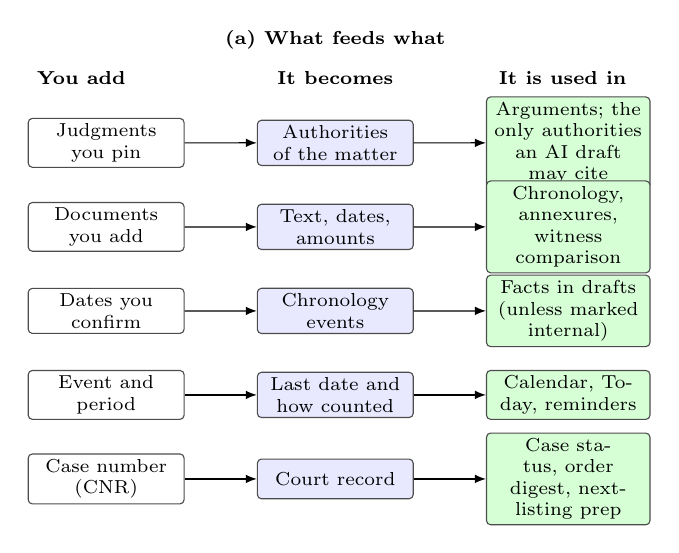
\begin{tikzpicture}[x=1cm,y=1cm,scale=0.97,transform shape]
\node[ttl] at (4.0,5.35) {(a) What feeds what};
\node[ttl, anchor=west] at (0.05,4.85) {You add};
\node[ttl] at (4.0,4.85) {It becomes};
\node[ttl, anchor=west] at (6.1,4.85) {It is used in};
\foreach \i/\y/\l/\m/\r in {1/4.0/{Judgments you pin}/{Authorities of the matter}/{Arguments; the only authorities an AI draft may cite},
                          2/2.9/{Documents you add}/{Text, dates, amounts}/{Chronology, annexures, witness comparison},
                          3/1.8/{Dates you confirm}/{Chronology events}/{Facts in drafts (unless marked internal)},
                          4/0.7/{Event and period}/{Last date and how counted}/{Calendar, Today, reminders},
                          5/-0.4/{Case number (CNR)}/{Court record}/{Case status, order digest, next-listing prep}} {
  \node[st, text width=1.9cm] (l\i) at (1.0,\y) {\l};
  \node[db, text width=1.9cm] (m\i) at (4.0,\y) {\m};
  \node[ok, text width=2.0cm] (r\i) at (7.05,\y) {\r};
  \draw[ar] (l\i)--(m\i); \draw[ar] (m\i)--(r\i);
}
\end{tikzpicture}
\end{minipage}%
\begin{minipage}[t]{0.48\textwidth}
\centering
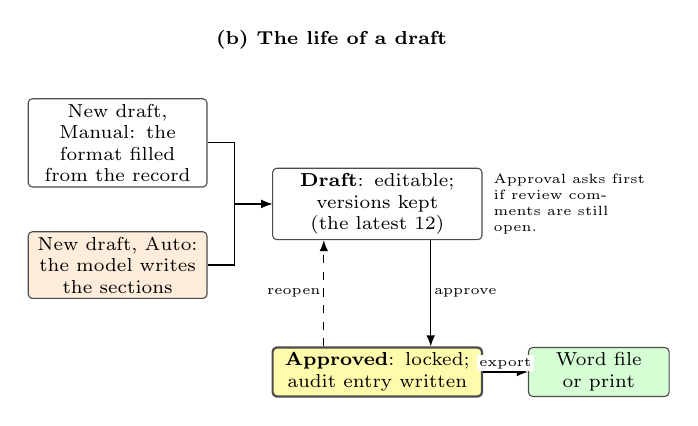
\begin{tikzpicture}[x=1cm,y=1cm,scale=0.97,transform shape]
\node[ttl] at (4.0,5.35) {(b) The life of a draft};
\node[st, text width=2.2cm] (m1) at (1.2,4.0) {New draft, Manual: the format filled from the record};
\node[ch, text width=2.2cm] (m2) at (1.2,2.4) {New draft, Auto: the model writes the sections};
\node[st, text width=2.6cm] (dr) at (4.6,3.2) {\textbf{Draft}: editable; versions kept (the latest 12)};
\node[hu, text width=2.6cm] (ap) at (4.6,1.0) {\textbf{Approved}: locked; audit entry written};
\node[ok, text width=1.7cm] (ex) at (7.5,1.0) {Word file or print};
\draw[ar] (m1.east) -- ++(0.35,0) |- (dr.west);
\draw[ar] (m2.east) -- ++(0.35,0) |- (dr.west);
\draw[ar] ([xshift=0.7cm]dr.south) -- node[lb, right]{approve} ([xshift=0.7cm]ap.north);
\draw[dar] ([xshift=-0.7cm]ap.north) -- node[lb, left]{reopen} ([xshift=-0.7cm]dr.south);
\draw[ar] (ap.east) -- node[lb, above]{export} (ex.west);
\node[font=\tiny, text width=2.0cm, align=left, anchor=west] at (6.0,3.2) {Approval asks first if review comments are still open.};
\end{tikzpicture}
\end{minipage}
\caption{(a) How the matter tabs feed each other: pinned authorities, confirmed dates and read documents flow into arguments and drafts. (b) A draft can be exported only after the advocate approves it; an approved draft is locked until reopened.}
\label{fig:pair1}
\end{figure*}


\section{Checks on Citations and on Model Text}
\label{sec:checks}
\textbf{The citation check} (Fig.~\ref{fig:checks}A) uses no model. It finds citations and case names by pattern, merges parallel citations, asks the index for each number and, failing that, searches by name with state abbreviations expanded (``M.P.'' and ``Madhya Pradesh'') and a one-letter spelling slip tolerated. It is simpler than the verifier of \S\ref{sec:verifier}, and, like it, confirms existence and not that a judgment supports the proposition.

\textbf{A model action} (Fig.~\ref{fig:checks}B) passes the advocate's text to the model as data and never as instructions. The reply must be valid JSON; a failed call is shown as an error and never replaced by a canned answer, and the percentages a model may offer for risk are not used. The reply is cleaned and then checked against sources. The cases it names are looked up in the index. A position attributed to a witness is kept only if its content words and every date and number in it appear in that witness's statement. A next hearing date is kept only if the order writes it. A chronology's source, and a document a witness is to be confronted with, must be documents that were supplied, and a dated event is kept only if the documents write its date. Items that fail are dropped and counted, the answer carries the model's name, and the advocate decides.

\begin{figure*}[t]
\centering
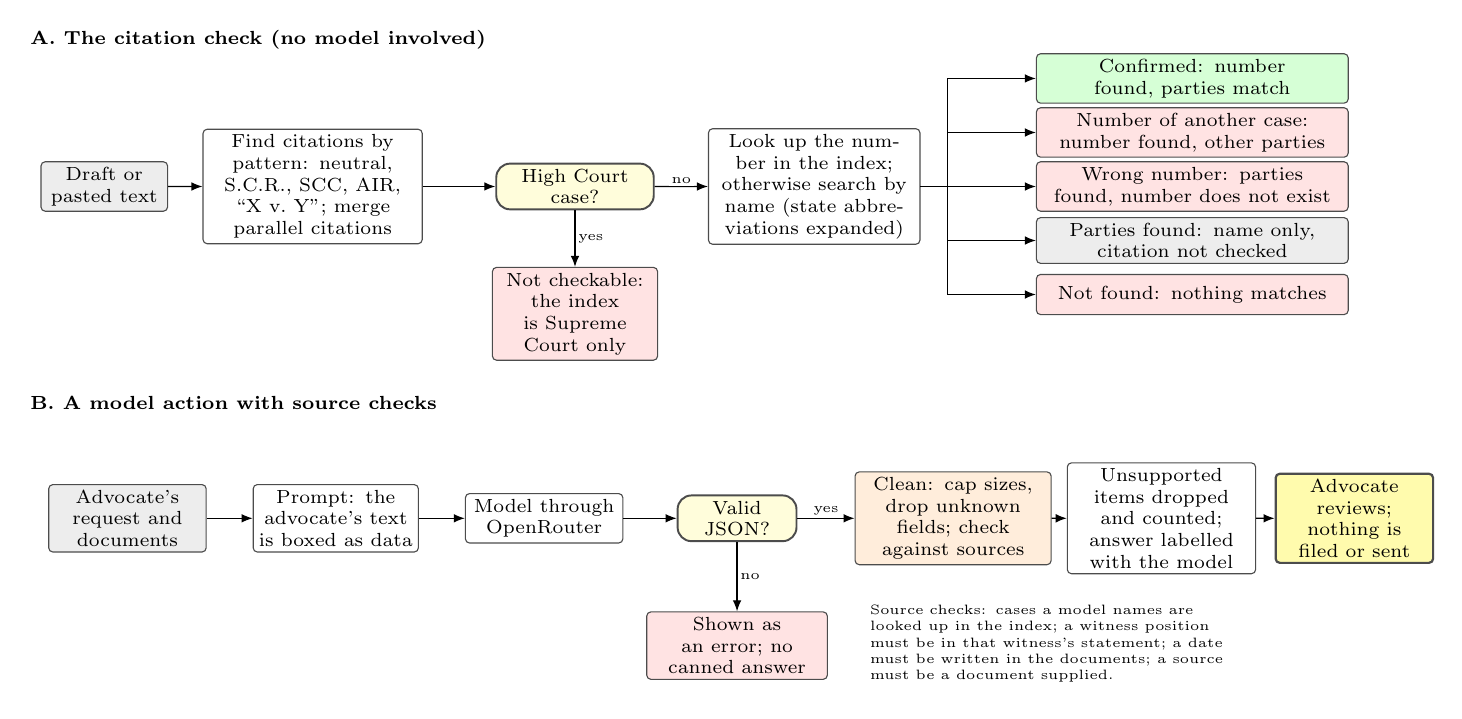
\begin{tikzpicture}[x=1cm,y=1cm,scale=0.98,transform shape]
% lane A: the citation check (no model involved)
\node[ttl, anchor=west] at (-0.2,4.5) {A. The citation check (no model involved)};
\node[io, text width=1.5cm] (c1) at (0.8,2.6) {Draft or pasted text};
\node[st, text width=2.7cm] (c2) at (3.5,2.6) {Find citations by pattern: neutral, S.C.R., SCC, AIR, ``X v.\ Y''; merge parallel citations};
\node[dec, text width=1.9cm] (c3) at (6.9,2.6) {High Court case?};
\node[st, text width=2.6cm] (c4) at (10.0,2.6) {Look up the number in the index; otherwise search by name (state abbreviations expanded)};
\node[wr, text width=2.0cm] (o0) at (6.9,0.95) {Not checkable: the index is Supreme Court only};
\node[ok, text width=3.9cm] (o1) at (14.9,4.0) {Confirmed: number found, parties match};
\node[wr, text width=3.9cm] (o2) at (14.9,3.3) {Number of another case: number found, other parties};
\node[wr, text width=3.9cm] (o3) at (14.9,2.6) {Wrong number: parties found, number does not exist};
\node[io, text width=3.9cm] (o4) at (14.9,1.9) {Parties found: name only, citation not checked};
\node[wr, text width=3.9cm] (o5) at (14.9,1.2) {Not found: nothing matches};
\draw[ar] (c1)--(c2); \draw[ar] (c2)--(c3); \draw[ar] (c3)--node[lb,above]{no}(c4); \draw[ar] (c3.south)--node[lb,right]{yes}(o0.north);
\foreach \o in {o1,o2,o3,o4,o5} { \draw[ar] (c4.east)--++(0.35,0)|-(\o.west); }
% lane B: a model action with source checks
\node[ttl, anchor=west] at (-0.2,-0.2) {B. A model action with source checks};
\node[io, text width=1.9cm] (g1) at (1.1,-1.7) {Advocate's request and documents};
\node[st, text width=2.0cm] (g2) at (3.8,-1.7) {Prompt: the advocate's text is boxed as data};
\node[st, text width=1.9cm] (g3) at (6.5,-1.7) {Model through OpenRouter};
\node[dec, text width=1.4cm] (g4) at (9.0,-1.7) {Valid JSON?};
\node[ch, text width=2.4cm] (g5) at (11.8,-1.7) {Clean: cap sizes, drop unknown fields; check against sources};
\node[wr, text width=2.2cm] (g6) at (9.0,-3.35) {Shown as an error; no canned answer};
\node[st, text width=2.3cm] (g7) at (14.5,-1.7) {Unsupported items dropped and counted; answer labelled with the model};
\node[hu, text width=1.9cm] (g8) at (17.0,-1.7) {Advocate reviews; nothing is filed or sent};
\draw[ar] (g1)--(g2); \draw[ar] (g2)--(g3); \draw[ar] (g3)--(g4); \draw[ar] (g4)--node[lb,above]{yes}(g5); \draw[ar] (g4.south)--node[lb,right]{no}(g6.north);
\draw[ar] (g5)--(g7); \draw[ar] (g7)--(g8);
\node[font=\tiny, text width=4.6cm, align=left, anchor=north west] at (10.6,-2.7) {Source checks: cases a model names are looked up in the index; a witness position must be in that witness's statement; a date must be written in the documents; a source must be a document supplied.};
\end{tikzpicture}
\caption{The two check pipelines of the workspace. (A) The citation check uses patterns and the index, never a model. (B) Every model action passes the advocate's text to the model as data, and what comes back is cleaned and checked against the advocate's own documents and the index before it is shown (\S\ref{sec:checks}).}
\label{fig:checks}
\end{figure*}


\section{Evidence, Dates and Drafts}
\label{sec:evidence}
\textbf{Evidence} (Fig.~\ref{fig:pair2}a) is read in the browser: text, Word and PDF files with a text layer directly, with pdf.js \cite{pdfjs}, and scans and photographs by Tesseract \cite{smith2007} in English, Hindi and Marathi. The files are not uploaded, and only their text is kept. Dates and rupee amounts, including Devanagari digits and month names, are found by pattern together with the nearest event word, and two documents that give different dates or amounts beside the same word are listed as possible inconsistencies: places to look, never findings. \textbf{Dates} (Fig.~\ref{fig:pair2}b): the calculator holds \CasePeriods{} periods, each naming its source (the Limitation Act, 1963 \cite{limitationact}, the Supreme Court Rules, 2013 \cite{scrules}, the Code of Civil Procedure and others). It leaves out the day of the event (s.\,12(1)) and, where the law allows it, the time taken to get a certified copy (s.\,12(2)), runs a period that ends on a closed day to the day the court reopens (s.\,4), and shows how the date was counted. \textbf{Drafts}: Manual fills one of \CaseFormats{} formats from the record and leaves a visible blank where the record has nothing. Auto (Fig.~\ref{fig:pair2}c) asks a model to write each section from the advocate's account and the record, under a prompt that allows only pinned authorities, only the matter's documents as annexures and a blank for a missing fact; the text is cleaned, every citation in it is looked up, and the earlier text is saved first as a version. A para-wise reply numbers the other side's paragraphs and builds the reply from a stance for each (admit, deny, partly, no knowledge, legal), leaving the substance to the advocate.

\begin{figure*}[t]
\centering
\begin{minipage}[t]{0.32\textwidth}
\centering
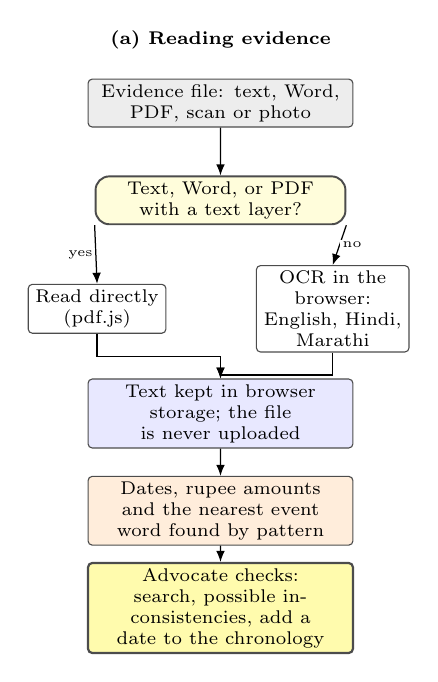
\begin{tikzpicture}[x=1cm,y=1cm,scale=0.95,transform shape]
\node[ttl] at (2.6,7.55) {(a) Reading evidence};
\node[io, text width=3.4cm] (e1) at (2.6,6.7) {Evidence file: text, Word, PDF, scan or photo};
\node[dec, text width=3.2cm] (e2) at (2.6,5.4) {Text, Word, or PDF with a text layer?};
\node[st, text width=1.7cm] (e3) at (0.95,3.95) {Read directly (pdf.js)};
\node[st, text width=1.9cm] (e4) at (4.1,3.95) {OCR in the browser: English, Hindi, Marathi};
\node[db, text width=3.4cm] (e5) at (2.6,2.55) {Text kept in browser storage; the file is never uploaded};
\node[ch, text width=3.4cm] (e6) at (2.6,1.25) {Dates, rupee amounts and the nearest event word found by pattern};
\node[hu, text width=3.4cm] (e7) at (2.6,-0.05) {Advocate checks: search, possible inconsistencies, add a date to the chronology};
\draw[ar] (e1)--(e2); \draw[ar] (e2.south west)--node[lb,left]{yes}(e3.north); \draw[ar] (e2.south east)--node[lb,right]{no}(e4.north);
\draw[ar] (e3.south)--++(0,-0.3)-|(e5.north); \draw[ar] (e4.south)--++(0,-0.3)-|(e5.north);
\draw[ar] (e5)--(e6); \draw[ar] (e6)--(e7);
\end{tikzpicture}
\end{minipage}\hfill
\begin{minipage}[t]{0.32\textwidth}
\centering
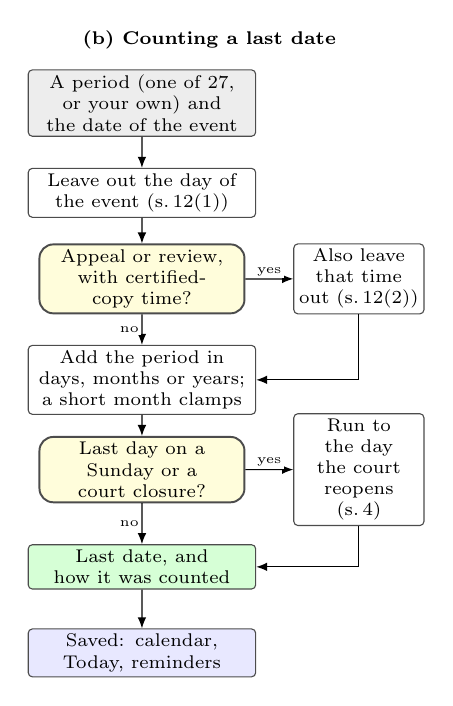
\begin{tikzpicture}[x=1cm,y=1cm,scale=0.95,transform shape]
\node[ttl] at (2.6,7.55) {(b) Counting a last date};
\node[io, text width=2.9cm] (l1) at (1.7,6.7) {A period (one of \CasePeriods{}, or your own) and the date of the event};
\node[st, text width=2.9cm] (l2) at (1.7,5.5) {Leave out the day of the event (s.\,12(1))};
\node[dec, text width=2.6cm] (l3) at (1.7,4.35) {Appeal or review, with certified-copy time?};
\node[st, text width=1.6cm] (l4) at (4.6,4.35) {Also leave that time out (s.\,12(2))};
\node[st, text width=2.9cm] (l5) at (1.7,3.0) {Add the period in days, months or years; a short month clamps};
\node[dec, text width=2.6cm] (l6) at (1.7,1.8) {Last day on a Sunday or a court closure?};
\node[st, text width=1.6cm] (l7) at (4.6,1.8) {Run to the day the court reopens (s.\,4)};
\node[ok, text width=2.9cm] (l8) at (1.7,0.5) {Last date, and how it was counted};
\node[db, text width=2.9cm] (l9) at (1.7,-0.65) {Saved: calendar, Today, reminders};
\draw[ar] (l1)--(l2); \draw[ar] (l2)--(l3);
\draw[ar] (l3)--node[lb,above]{yes}(l4); \draw[ar] (l3)--node[lb,left]{no}(l5);
\draw[ar] (l4.south) |- (l5.east);
\draw[ar] (l5)--(l6);
\draw[ar] (l6)--node[lb,above]{yes}(l7); \draw[ar] (l6)--node[lb,left]{no}(l8);
\draw[ar] (l7.south) |- (l8.east);
\draw[ar] (l8)--(l9);
\end{tikzpicture}
\end{minipage}\hfill
\begin{minipage}[t]{0.32\textwidth}
\centering
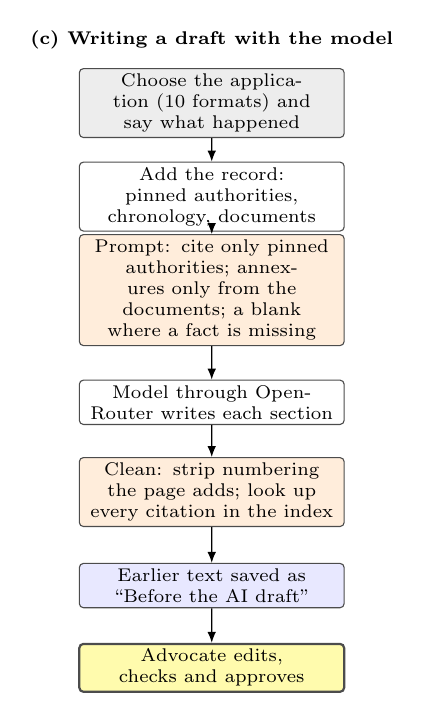
\begin{tikzpicture}[x=1cm,y=1cm,scale=0.95,transform shape]
\node[ttl] at (2.6,7.55) {(c) Writing a draft with the model};
\node[io, text width=3.4cm] (d1) at (2.6,6.7) {Choose the application (\CaseFormats{} formats) and say what happened};
\node[st, text width=3.4cm] (d2) at (2.6,5.45) {Add the record: pinned authorities, chronology, documents};
\node[ch, text width=3.4cm] (d3) at (2.6,4.2) {Prompt: cite only pinned authorities; annexures only from the documents; a blank where a fact is missing};
\node[st, text width=3.4cm] (d4) at (2.6,2.7) {Model through OpenRouter writes each section};
\node[ch, text width=3.4cm] (d5) at (2.6,1.5) {Clean: strip numbering the page adds; look up every citation in the index};
\node[db, text width=3.4cm] (d6) at (2.6,0.25) {Earlier text saved as ``Before the AI draft''};
\node[hu, text width=3.4cm] (d7) at (2.6,-0.85) {Advocate edits, checks and approves};
\draw[ar] (d1)--(d2); \draw[ar] (d2)--(d3); \draw[ar] (d3)--(d4); \draw[ar] (d4)--(d5); \draw[ar] (d5)--(d6); \draw[ar] (d6)--(d7);
\end{tikzpicture}
\end{minipage}
\caption{Three processes of the workspace. (a) Evidence is read where it lies and only its text is kept. (b) A limitation date is counted by stated rules and shows its steps (\S\ref{sec:system}). (c) An AI draft is bound to the matter's own record and is a draft for the advocate, not a filing.}
\label{fig:pair2}
\end{figure*}


\section{A Worked Case}
\label{sec:case}
We ran the workspace on a real Supreme Court case, \emph{Rajendra S/o Ramdas Kolhe v.\ State of Maharashtra} (Criminal Appeal No.~2281 of 2011, decided 15 May 2024, 2024~INSC~422), a murder appeal that turns on a dying declaration. The judgment, the Court's summaries of the six prosecution witnesses, the orders it recites and a draft written for this test are in \texttt{sample-case/}; the scripts that produce every number below are in \texttt{paper/final/case\_study/}.

\textbf{Reading and dates.} The Evidence tab read the judgment (\CaseJudgWords{} words) and found \CaseJudgDates{} dates and \CaseJudgAmounts{} amount; ``Ex.~59'', the deceased's written dying declaration, occurs \CaseJudgExhibit{} times in it and \CaseStmtExhibit{} in the witness summaries (\CaseStmtWords{} words). The three documents give no conflicting dates or amounts, so the list of possible inconsistencies is empty. For a review petition (Order~XLVII Rule~2, Supreme Court Rules, 2013 \cite{scrules}) the calculator, given \CaseLimitStart, returns \CaseLimitDate{} and shows that the day of the judgment is left out.

\textbf{Checking a draft.} The draft is a few paragraphs of submissions into which we planted errors (Table~\ref{tab:case}). The citation check found \CaseCiteFound{} cases. Of these, \CaseCiteVerified{} were confirmed. One has the right parties and a wrong volume (\emph{Paniben}, cited as [1992] 9 S.C.R.\ 197, reported at [1992] 2 S.C.R.\ 197). One gives the appellant's own case the number of \emph{Khushal Rao v.\ State of Bombay}. One, \emph{Verma v.\ State of Karnataka}, does not exist. One is a High Court case, reported as not checkable. We planted the errors, so this shows that the check catches those kinds of error, not how often they occur. The case also exposed three defects in how the check searches the index (a state written in full where the archive writes ``M.P.'', a party name matched to a different case, and a spelling slip in a title); we fixed them and added regression tests. One limit remains: \emph{Sudhakar v.\ State of Madhya Pradesh}, which the archive spells ``Shudhakar'', is found by its number but not by name, because the index is searched by whole words.

\begin{table}[t]
\caption{The draft with planted errors and what the citation check reported.}
\label{tab:case}
\centering
\footnotesize
\setlength{\tabcolsep}{3pt}
% GENERATED by case_study/make_case_tex.mjs. Do not edit.
\begin{tabular}{@{}>{\raggedright\arraybackslash}p{1.3in}>{\raggedright\arraybackslash}p{0.95in}>{\raggedright\arraybackslash}p{0.85in}@{}}
\toprule
Case as cited & Citation & Verdict \\
\midrule
Khushal Rao v. State of Bombay & [1958] 1 S.C.R. 552 \textperiodcentered{} 1957 INSC 79 & Confirmed \\
Ashabai v. State of Maharashtra & [2013] 1 S.C.R. 115 & Confirmed \\
Lakhan v. State of Madhya Pradesh & [2010] 9 S.C.R. 705 \textperiodcentered{} 2010 INSC 489 & Confirmed \\
Paniben (Smt.) v. State of Gujarat & [1992] 9 S.C.R. 197 & Wrong number \\
Sher Singh v. State of Punjab & 2008 INSC 204 & Confirmed \\
Rajendra Kolhe v. State of Maharashtra & [1958] 1 S.C.R. 552 & Number of another case \\
Verma v. State of Karnataka & [2011] 5 S.C.R. 410 & Not found \\
State v. Rao & (name only) & High Court, not checkable \\
\bottomrule
\end{tabular}

\end{table}

\textbf{Checks on model text.} We sent the real prompts of three model actions that read these documents to \GroundModel, one of the four models of \S\ref{sec:setup}, three times each (temperature 0.2, seeds 1--3, a context of 8{,}192 tokens), kept its raw answers, and counted what the source checks removed. The witness comparison returned \GroundMatrixProposed{} points in \GroundMatrixRuns{} runs (\GroundMatrixEmptyRuns{} run returned none); the checks dropped \GroundMatrixDropped, a point whose second side named no witness, and kept \GroundMatrixKept, which quote the statements faithfully. The checks test fidelity to the source, not whether two statements conflict, and whether a kept point is a contradiction an advocate could use is a legal judgment we do not make. In all \GroundDigestRuns{} runs the order digest gave a next hearing date, \GroundDigestDates, worked out from ``two weeks from today''; the order writes none, and each was replaced by ``not stated in the order''. The chronology proposed \GroundTimelineProposed{} dated events, and \GroundIsoMissing{} of \GroundIsoProposed{} dates were not in the documents, so their events were dropped. The model named \GroundSourcesNamed{} sources and \GroundQDocsNamed{} documents to confront a witness with, and \GroundSuppliedClause. The context had to be 8{,}192 tokens: at Ollama's default of 4{,}096 the chronology prompt, of about 4{,}000 tokens, left room for only 100 tokens of answer. This is one case, one small model and three runs per action; it shows that the checks remove what the documents do not support, not how often a larger or hosted model would produce it.

\section{Limitations and Ethics}
\label{sec:discussion}
\textbf{Limitations.} VakilBuddy is a prototype: its matters other than the worked case are sample data, its court-status service answers from sample pages, its citation check is simpler than the evaluated verifier, and the workspace is covered by \CaseTestsWorkspace{} automated tests and its index service by \CaseTestsApi{}, not by a user study, so we make no claim about drafting quality or time saved. On one laptop, exact lookups in the index take a median of \LatExactMedian\,ms and the verifier \VerifyMedianMs\,ms.

\textbf{Ethics.} The workspace is decision support: the advocate remains responsible to the court, nothing is filed or sent by the workspace, every model answer is labelled and every draft needs approval. Evidence files are read in the browser and not uploaded, but the text of the documents an advocate sends to a model action goes to the model provider, which matters for privileged material. An AI assistant was used to build the software and draft this paper, as the acknowledgment states.

\section{Conclusion}
\label{sec:conclusion}
Indian courts now treat reliance on fabricated precedents as misconduct \cite{gummadi}, so a model-drafted citation must be checked before it reaches a court. From open data we built an audited index of \CorpusTotal{} judgments and orders, a verifier whose labels were correct in \AuditPct{} of a held-out audit, and an open citation graph of \GraphEdges{} links. Small open models answering from memory fabricate freely; an existence check removes the fabricated cases but not the lack of authority; search by subject over headnotes, ranked with the graph's citation counts, raised the share of questions answered with a deciding judgment from \RefRateClosed{} to \RefRateTopicPrior{} while \VerPctAllTopicPrior{} of the listed cases were verified. VakilBuddy applies these checks and an approval gate in an advocate's workspace, and a worked Supreme Court case shows them catching planted citation errors and unsupported model output. Connecting the evaluated retriever to the workspace, benchmarking the hosted models it calls, and measuring what it saves an advocate remain open.


\section*{Acknowledgment}
An AI assistant (Claude, Anthropic) was used to write the software, run the experiments and analyses, produce the first-pass labels of the verifier audit, the manual check of the citation graph and the reference answers for T4, and draft the text. The authors are responsible for the content.

\section*{Data and Code Availability}
The index builder, repair scripts, verifier, citation extractor, citation graph (every resolved and unresolved citation with its resolution tier), headnote embeddings, retrieval code, benchmark items, prompts, raw model outputs, scoring code, the workspace and the worked-case scripts and files are available from the authors. The underlying data are CC-BY-4.0 \cite{awssc,awshc}.

\bibliographystyle{IEEEtran}
\bibliography{refs,refs_extra}

\end{document}
